%
% Documento: Fundamenta\c{c}\~{a}o
%

\chapter{FUNDAMENTA\c{c}\~{a}O}\label{chap:fundamentacao}

Neste cap\'{i}tulo apresentaremos as pesquisas bibliogr\'{a}ficas, para a fundamenta\c{c}\~{a}o te\'{o}rica que nos permite termos a base para alcan\c{c}ar os objetivos estabelecidos para este trabalho.

Al\'{e}m dos principais conceitos sobres os temas abordados neste trabalho como: Sistemas de informa\c{c}\~{a}o, BI, conhecimentos sobre fontes de dados, ETL, DW, DM, KDD, OLAP, Cubo, Data mining e um hist\'{o}rico sobre o servi\c{c}o 181 (disque denúncia) s\~{a}o necess\'{a}rios para a aplica\c{c}\~{a}o, desenvolvimento de um BI funcional e bem dimensionado.

\section{Sistemas de informa\c{c}\~{a}o}

Um sistema de informa\c{c}\~{a}o \'{e}um conjunto interdependente de pessoas, estruturas organizacionais, software, hardware, processos e m\'{e}todos interligados com o objetivo de facilitar o planejamento e o controle em empresas e outras organiza\c{c}\~{o}es, organizando informa\c{c}\~{o}es de forma que estas se tornem utiliz\'{a}veis na coordena\c{c}\~{a}o do fluxo de trabalho de uma empresa \cite{si-laudon-laudon}.

\subsection{SPT (Sistemas de processamento de transa\c{c}\~{o}es)}

Os sistemas de processamento de transa\c{c}\~{o}es, representam a aplica\c{c}\~{a}o dos conceitos e tecnologia de informa\c{c}\~{a}o em transa\c{c}\~{o}es rotineiras, repetitivas e geralmente comuns de neg\'{o}cios \cite{si-stair-1998}. Uma transa\c{c}\~{a}o pode ser entendida como um evento que ocorre num neg\'{o}cio tal como compra, venda, pagamento, entre outros.

Os sistemas de processamento de transa\c{c}\~{o}es possuem foco no n\'{i}vel operacional da empresa, armazenando e processando fluxos de dados pertinentes a automa\c{c}\~{a}o de processos de modo que estes sejam mais planejados e otimizados, visando garantir a integra\c{c}\~{a}o e normaliza\c{c}\~{a}o, possuindo, em sua grande maioria, alguns relat\'{o}rios para gerenciamento.

\subsection{SIG (Sistemas de informa\c{c}\~{o}es gerenciais)}

Sistema de Informa\c{c}\~{a}o Gerencial \'{e}o processo de transforma\c{c}\~{a}o de dados em informa\c{c}\~{o}es que ser\~{a}o utilizadas na estrutura decis\'{o}ria da empresa, bem como proporcionar\~{a}o a sustenta\c{c}\~{a}o administrativa para otimizar os resultados esperados \cite{si-oliveira-1998}.

\begin{flushleft}
	Estes sistemas têm o prop\'{o}sito de fornecer informa\c{c}\~{o}es necess\'{a}rias \`{a} medi\c{c}\~{a}o da eficiência operacional da organiza\c{c}\~{a}o, dando ênfase \`{a}s necessidades gerenciais atrav\'{e}s de informa\c{c}\~{o}es resumidas, obtidas a partir da filtragem e an\'{a}lise de dados altamente detalhados, extra\'{i}dos das bases de dados dos sistemas de processamento transacionais e de fontes \cite{si-stair-1998} \cite{si-falsarella-chaves-1998}.
\end{flushleft}

\subsection{SAD (Sistemas de apoio \`{a} decis\~{a}o)}

Os Sistemas de Apoio \`{a} Decis\~{a}o, s\~{a}o sistemas que realizam o processamento anal\'{i}tico e provêem as informa\c{c}\~{o}es necess\'{a}rias ao usu\'{a}rio, permitindo a an\'{a}lise de situa\c{c}\~{o}es e a tomada de decis\~{o}es \cite{si-inmon-1997}.

Os processamentos anal\'{i}ticos dos SAD permitem ao usu\'{a}rio analisar uma grande quantidade de dados, normalmente hist\'{o}ricos, verificando problemas e situa\c{c}\~{o}es, de modo a identificar perfis, tendências e padr\~{o}es, sendo a performance das consultas ou extra\c{c}\~{o}es de dados importantes, por\'{e}m n\~{a}o crucial no desenvolvimento deste tipo de aplica\c{c}\~{a}o.

\subsection{SIE (Sistemas de informa\c{c}\~{a}o executiva)}

Os Sistemas de Informa\c{c}\~{a}o executiva, s\~{a}o um tipo especial de SAD destinado \`{a} tomada de decis\~{o}es de alto n\'{i}vel da organiza\c{c}\~{a}o, oferecendo informa\c{c}\~{o}es estruturadas, tanto internas quanto externas a respeito de aspectos da organiza\c{c}\~{a}o considerados fatores \cite{si-stair-1998} \cite{si-falsarella-chaves-1998}.

Enquanto um SAD oferece apoio para decis\~{o}es focadas em uma \'{a}rea espec\'{i}fica, geralmente oferecendo suporte \`{a} m\'{e}dia e baixa gerência, um EIS (Executive Information Systems) oferece informa\c{c}\~{o}es consolidadas de alto n\'{i}vel e an\'{a}lises multidimensionais para os executivos de alto n\'{i}vel \cite{si-gupta-2001}.

\section{BI (Business Intelligence)}

A Origem do Termo \textit{Business Intelligence} (BI) foi utilizado pela primeira vez na d\'{e}cada de 50 por Hans Peter Luhn, um pesquisador da IBM, no artigo intitulado “A Business Intelligence System” \cite{bi-elena-2011}. O autor prop\~{o}e o desenvolvimento de sistema autom\'{a}tico, baseado em m\'{a}quinas de processamento de dados, que indexa e codifica automaticamente documentos e dissemina informa\c{c}\~{o}es nas organiza\c{c}\~{o}es conforme o ponto de a\c{c}\~{a}o.

Assim em 1989, \textit{Howard Dresner}, um membro de pesquisa do \textit{Gartner Group} popularizou “BI” com um termo gen\'{e}rico, usado para descrever um conjunto de conceitos e m\'{e}todos para aperfei\c{c}oar a tomada de decis\~{o}es de neg\'{o}cios utilizando sistemas de suporte baseados em fatos.

Dresner deixou o \textit{Gartner} em 2005 e entrou para a \textit{Hyperion Soluctions} como seu CSO (\textit{Chief Strategic Officer} – Diretor de Estrat\'{e}gia).

J\'{a} \cite{bi-cortes-2008} afirma que o \textit{Business Intelligence} (BI ou intelig\^{e}ncia empresarial) est\'{a} relacionado \`{a} habilidade de compreender, entender e ter o conhecimento necess\'{a}rio do pr\'{o}prio neg\'{o}cio de modo que as suposi\c{c}\~{o}es possam ser realizadas com grande chance de sucesso e que possam ter resultados satisfat\'{o}rios.

Para \cite{dw-kimball-2013} o sistema DW/BI deve tornar as informa\c{c}\~{o}es facilmente acess\'{i}veis. O conteúdo do sistema DW/BI deve ser compreens\'{i}vel. Os dados devem ser intuitivos e \'{o}bvios para o usu\'{a}rio comercial, n\~{a}o apenas para o desenvolvedor. As estruturas e os r\'{o}tulos dos dados devem imitar os processos e o vocabul\'{a}rio dos usu\'{a}rios de neg\'{o}cios. Os usu\'{a}rios corporativos desejam separar e combinar dados anal\'{i}ticos em infinitas combina\c{c}\~{o}es.

Em s\'{i}ntese, na figura abaixo, h\'{a} uma descri\c{c}\~{a}o como o BI pode ser entendido, como uma metodologia que permite transformar dados em informa\c{c}\~{o}es qualificadas, gerando conhecimento para a tomada de decis\~{o}es.

\begin{figure}[H]
	\vspace*{0,2cm}
    \centering
    \caption{Ilustra\c{c}\~{a}o da estrutura}
    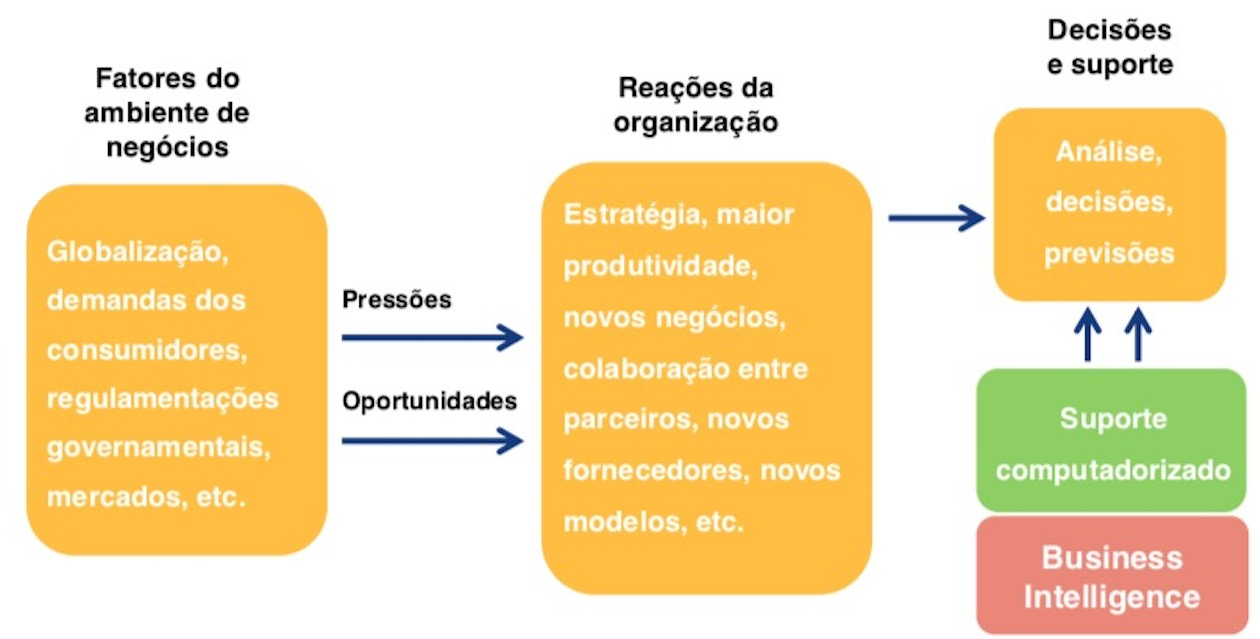
\includegraphics[width=0.6\textwidth]{./04-figuras/figura-01}
    \label{fig:ilustfig01}
\end{figure}
\vspace*{-0,9cm}
{\raggedright \fonte{Dispon\'{i}vel em: <https://Portal (www.fp2.com.br)>. Acesso em: 10 ago. 2020.}}\\

\subsection{A arquitetura e componentes}

Como j\'{a} mencionado temos como base os estudos de \cite{dw-kimball-2013}, seus elementos de arquitetura est\~{a}o representados na figura abaixo, como ilustrado, para \cite{dw-kimball-2013}, existem quatro componentes separados e distintos a serem considerados no ambiente DW/BI: sistemas de origem operacional, sistema ETL, \'{a}rea de apresenta\c{c}\~{a}o de dados e aplicativos de intelig\^{e}ncia de neg\'{o}cios.

\begin{figure}[H]
	\vspace*{0,2cm}
    \centering
    \caption{Elementos principais da arquitetura Kimball DW/BI.}
    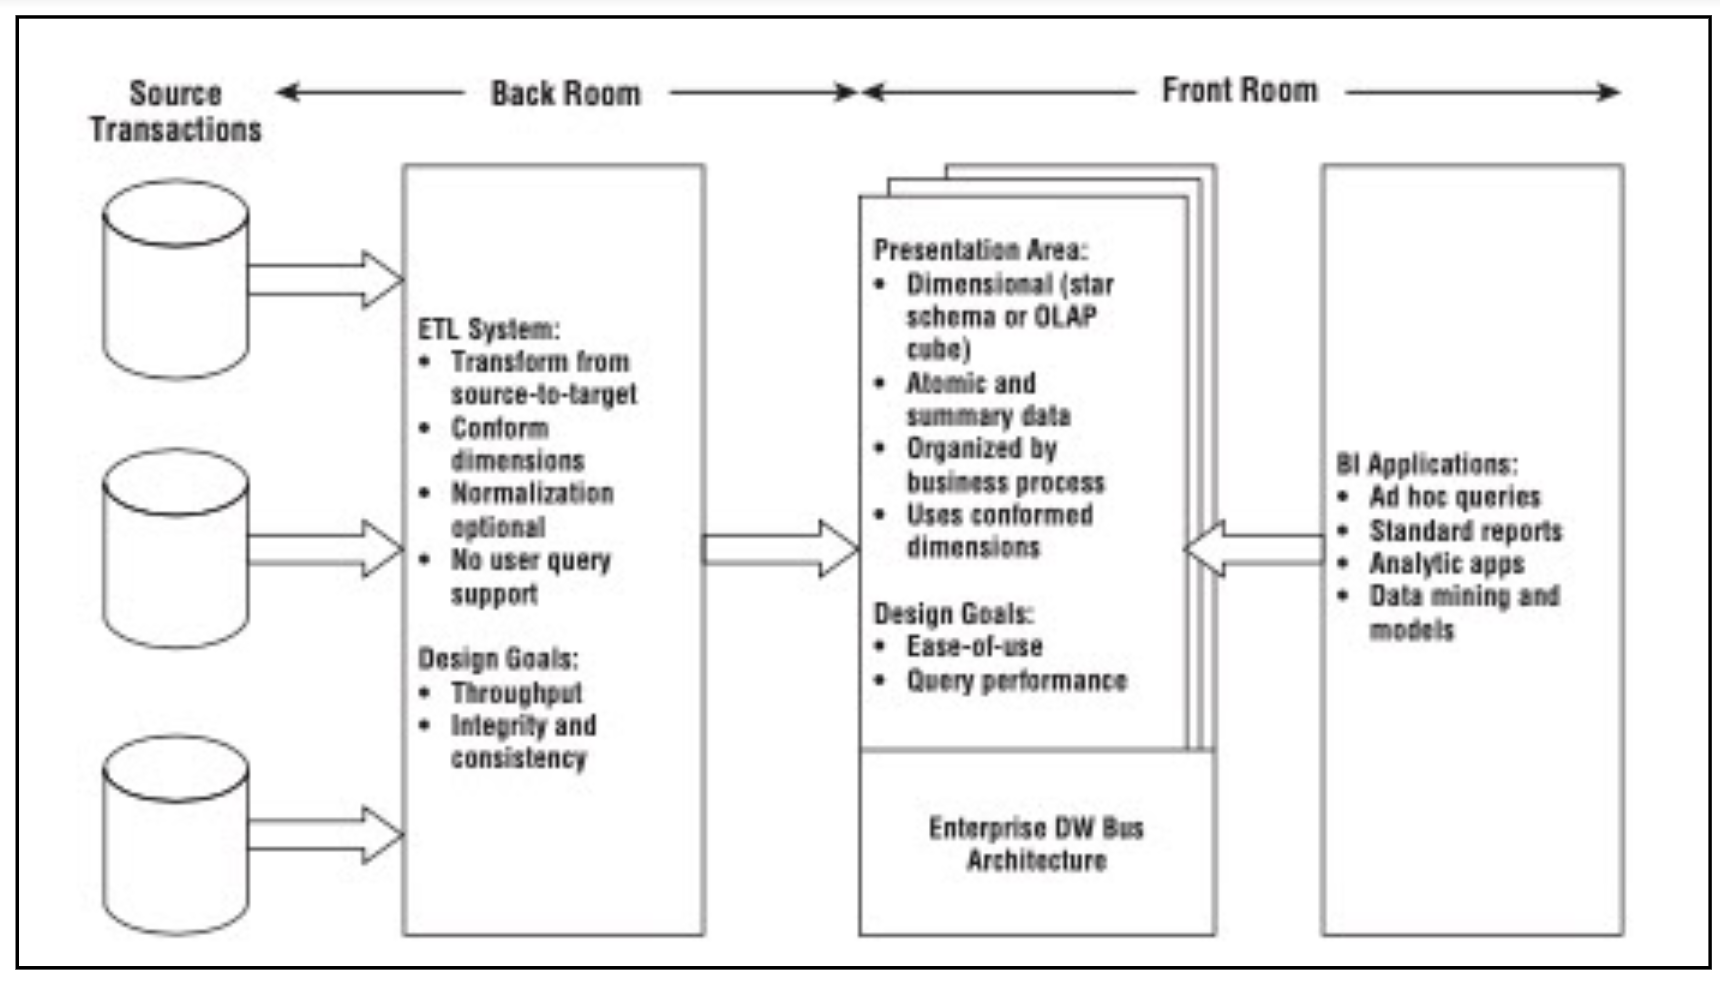
\includegraphics[width=0.6\textwidth]{./04-figuras/figura-02}
    \label{fig:ilustfig02}
\end{figure}
\vspace*{-0,9cm}
{\raggedright \fonte{ \textit{Core elements of the Kimball DW/BI architecture,} \cite{dw-kimball-1998}}}\\

O primeiro dele \'{e} o \textit{Operational Source Systems} que s\~{a}o os sistemas operacionais de registro ou origem que capturam as transa\c{c}\~{o}es da empresa. Pense nos sistemas de origem como fora do \textit{Data Warehouse}, porque, presumivelmente voc\^{e} tem pouco ou nenhum controle sobre o conteúdo e o formato dos dados nesses sistemas operacionais. 

As principais prioridades dos sistemas de origem s\~{a}o o desempenho e a disponibilidade do processamento. As consultas operacionais em rela\c{c}\~{a}o aos sistemas de origem s\~{a}o consultas estreitas, um registro por vez, que fazem parte do fluxo normal da transa\c{c}\~{a}o e severamente restringidas em suas demandas no sistema operacional.

O segundo \'{e} o ETL (\textit{Extract, Transformation, and Load System}) s\~{a}o os sistemas respons\'{a}veis pela: extra\c{c}\~{a}o, transforma\c{c}\~{a}o e carregamento. E que consiste em uma \'{a}rea de trabalho, estruturas de dados instanciadas e um conjunto de processos.

A cria\c{c}\~{a}o de estruturas normalizadas para o ETL e estruturas dimensionais para apresenta\c{c}\~{a}o, significa que os dados s\~{a}o potencialmente extra\'{i}dos, transformados e carregados duas vezes - uma vez no banco de dados normalizado e depois novamente quando voc\^{e} carrega o modelo dimensional. 

A terceira \'{e} \textit{Presentation Area to Support Business Intelligence} \'{e} nela onde os dados s\~{a}o organizados, armazenados e disponibilizados para consulta direta por usu\'{a}rios, redatores de relat\'{o}rios e outros aplicativos de BI anal\'{i}ticos.

A quarta \'{e} o \textit{Business Intelligence Applications} que \'{e} o componente final da arquitetura Kimball DW/BI. \'{e} o aplicativo de \textit{Business Intelligence} (BI) composto de uma variedade de recursos fornecidos aos usu\'{a}rios de neg\'{o}cios para alavancar a \'{a}rea de apresenta\c{c}\~{a}o para tomada de decis\~{a}o anal\'{i}tica.

Um aplicativo de BI pode ser t\~{a}o simples quanto uma ferramenta de consulta \textit{ad hoc} ou t\~{a}o complexo quanto um aplicativo sofisticado de minera\c{c}\~{a}o ou modelagem de dados. 

As ferramentas de consulta \textit{ad-hoc}, por mais poderosas que sejam, podem ser entendidas e usadas efetivamente apenas por uma pequena porcentagem da popula\c{c}\~{a}o potencial de usu\'{a}rios de neg\'{o}cios de DW/BI. 

Alguns dos aplicativos mais sofisticados, como ferramentas de modelagem e previs\~{a}o, podem fazer \textit{upload} de resultados de volta para os sistemas operacionais de origem, sistema ETL ou \'{a}rea de apresenta\c{c}\~{a}o.

\subsection{N\'{i}veis organizacionais}

Por padr\~{a}o as organiza\c{c}\~{o}es adotam abordagem de BI que abrange os tr\^{e}s n\'{i}veis hier\'{a}rquicos da organiza\c{c}\~{a}o: estrat\'{e}gico, t\'{a}tico e operacional. O BI tradicional, tamb\'{e}m conhecido como BI 1.0, abrange apenas os n\'{i}veis estrat\'{e}gico e  t\'{a}tico. Por\'{e}m, o uso de BI tamb\'{e}m pode ser usado no n\'{i}vel operacional, \cite{bi-imhoff-2006}, \cite{bi-airinei-2009}, \cite{bi-baltzan-2012}, \cite{bi-turban-2013}

Segundo \cite{bi-turban-2013}) a alta competitividade \'{e} o principal fator que influ\^{e}ncia empresas a adotarem BI no n\'{i}vel operacional.

Nesse n\'{i}vel de competi\c{c}\~{a}o tamb\'{e}m se busca melhorar decis\~{o}es, como dar respostas mais r\'{a}pidas aos clientes. 

O Quadro abaixo, apresenta um comparativo entre os tipos de BI. Na primeira coluna, \'{e}apresentada a carater\'{i}stica a ser comparada. Na segunda, como essa caracter\'{i}stica \'{e}vista no BI estrat\'{e}gico. Na terceira, como \'{e}no BI t\'{a}tico. Por fim, na última, como \'{e}no BI operacional.

A principal diferen\c{c}a est\'a{a} na temporalidade dos dados e no foco de neg\'{o}cio. O BI operacional deve ser imediato ou no mesmo dia e objetiva auxiliar o controle das opera\c{c}\~{o}es di\'{a}rias \cite{bi-turban-2013}. Mesmo  assim, \'{e} importante que os três tipos sejam orientados e alinhados aos objetivos da organiza\c{c}\~{a}o \cite{bi-baltzan-2012}.

\begin{quadro}[H]
	\begin{center}
		\caption{Comparativo entre as Características do BI Operacional, T\'{a}tico e Estratégico..\label{qua:quadro-01}}
	    \begin{tabular}{ |p{3cm}|p{3cm}|p{3cm}|p{3cm}| }
			\hline
		    Caracter\'{i}sticas & 
            BI Operacional & 
            BI T\'{a}tico & 
            BI Estrat\'{e}gico \\
		    \hline
            Foco principal do neg\'{o}cio &
            Administrar operações do dia a dia &
            Analisar dados; entregar relatórios & 
            Atingir as metas empresariais e longo prazo \\
            \hline
            Principais usu\'{a}rios &
            Gerente de setor &
            Executivos, analistas, gerentes de setor &
            Executivos, analistas \\
            \hline
            M\'{e}tricas &
            Métricas são individualizadas 
            para que o gestor de cada linha
            possa obter insight sobre o
            desempenho de seus processos de negócio
            &
            Métricas são um mecanismo de \textit{feedback}
            para companhar e entender como a estratégia
            está progredindo e quais ajustes precisam ser planejada
            &
            Métricas são um mecanismo de \textit{feedback}
            para companhar e entender como a
            estratégia está progredindo e quais ajustes
            precisam ser planejados
            \\
            \hline
            Prazo &
            Imediatamente, dentro do dia &
            Diário, semanal, mensal&
            Mensal, trimestral, anual \\
            \hline
            Tipos de dados ou usos  &
            Em tempo real ou quase em tempo real  &
            Histórico, preditivo  &
            Histórico, preditivo \\
            \hline
    	\end{tabular}
	\end{center}
	\vspace*{-0,8cm}
	{\raggedright \fonte{Elaborado à partir de\cite{bi-turban-2013}}
\end{quadro}

\subsection{\textit{Next Generation Business Intelligence} ou BI 2.0}

Pode-se dizer que a tecnologia de \testint{Business Intelligence} n\~{a}o disp\~{o}e de um conceito pr\'{e}-definido, ou seja, pode ser compreendida e explicada de diversas formas, o mesmo acontece com a \textit{Next Generation Business Intelligence}, muito embora sejam utilizados conceitos bem parecidos na sua defini\c{c}\~{a}o. 

O BI da segunda gera\c{c}\~{a}o concentra-se mais no contexto de fluxos de dados e no conhecimento, e n\~{a}o apenas nas informa\c{c}\~{o}es como o BI de primeira gera\c{c}\~{a}o. Ou seja, o BI 2.0 \'{e} como uma extens\~{a}o da Web 2.0 no cen\'{a}rio empresarial, tornando-se uma oportunidade importante para o usu\'{a}rio e ampliando os conhecimentos sobre a camada de apresenta\c{c}\~{a}o, visualiza\c{c}\~{a}o de dados e informa\c{c}\~{o}es sobre a demanda. 

Dados estruturados e n\~{a}o estruturados, empresarial e público, que incluem novos relat\'{o}rios de an\'{a}lise e intera\c{c}\~{a}o.

O principal benef\'{i}cio do \textit{Next Generation Business Intelligence} para uma organiza\c{c}\~{a}o \'{e} a capacidade de fornecer informa\c{c}\~{o}es precisas quando necess\'{a}rio, incluindo uma vis\~{a}o em tempo real do desempenho corporativo. Para permitir adaptar os modelos de neg\'{o}cios para o mundo de hoje em tempo real, aplica\c{c}\~{o}es de software s\~{a}o criadas agora utilizando ED \testint{(event-driven)}, ou seja, dirigido a eventos. 

Assim os dados se movem em tempo real sobre arquiteturas orientadas a servi\c{c}os, utilizando servi\c{c}os de baixo acoplamento e altamente interoper\'{a}veis, ou seja, operacional em servi\c{c}os de v\'{a}rias formas, que promovem a integra\c{c}\~{a}o de aplicativos padronizados.

Na pr\'{o}xima figura, est\'{a} ilustrado os principais componentes de um sistema de \textit{Next Generation Business Intelligence} e uma breve explana\c{c}\~{a}o sobre cada um:

\begin{figure}[H]
	\vspace*{0,2cm}
    \centering
    \caption{Componentes de um sistema de BI 2.0.}
    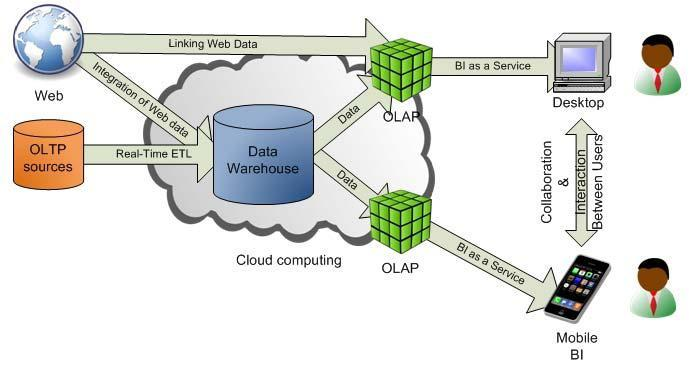
\includegraphics[width=0.6\textwidth]{./04-figuras/figura-03}
    \label{fig:ilustfig03}
\end{figure}
\vspace*{-0,9cm}
{\raggedright \fonte{Dispon\'{i}vel em: Portal (www.devmedia.com.br), Processo de Cria\c{c}\~{a}o e Exposi\c{c}\~{a}o, dispon\'{i}vel em: <https://www.devmedia.com.br/business-intelligence-2-0-conceitos-componentes-e-arquitetura/28899>, acessado em 5 jun de 2020.}}\\

Na figura acima nota-se que o BI 2.0 extrai dados n\~{a}o somente de um DW, mas sim de dados on-line e em tempo real com o aux\'{i}lio do OLTP (On-line Transaction Processing) e do Real Time ETL (Processo ETL em tempo real).

A seguir uma breve explica\c{c}\~{a}o sobre cada um de seus componentes. O bom est\'{a} ciente de que al\'{e}m das fontes de dados tradicionais, ou seja, transa\c{c}\~{a}o de dados, as fontes de dados de BI est\~{a}o evoluindo para incluir at\'{e} mesmo os mensagens enviadas por intranets empresariais e perfis pessoais de funcion\'{a}rios e clientes da web. Os dispositivos m\'{o}veis e outros dados do sensor tamb\'{e}m s\~{a}o adicionados \`{a}s fontes de dados. Contudo, muitas dessas fontes de dados n\~{a}o s\~{a}o estruturadas. Para isto precisamos entender as tecnologias:

\begin{itemize}

    \item Web 2.0: Novas pr\'{a}ticas e abordagens da web com conteúdo dinâmicos e ass\'{i}ncronos\index{NewR}\footnote{Ass\'{i}ncronos: na \'{a}rea da tecnologia da informa\c{c}\~{a}o, a comunica\c{c}\~{a}o ass\'{i}ncrona \'{e} a transmiss\~{a}o de dados, geralmente sem o uso de um sinal de rel\'{o}gio externo, onde os dados podem ser transmitidos intermitentemente em um fluxo est\'{a}vel.} que possibilitam os usu\'{a}rios interagirem com a p\'{a}gina e com outros usu\'{a}rios, ex: Redes Sociais;
    
    \item OLTP (\textit{Online Transaction Processing}):, ou seja, processamento de transa\c{c}\~{o}es em tempo real. S\~{a}o sistemas que registram as transa\c{c}\~{o}es, como, por exemplo, os ERPs (\textit{Enterprise Resource Planning});
    
    \item \textit{Real Time ETL}: Processo de extra\c{c}\~{a}o, transforma\c{c}\~{a}o e carga de dados em tempo real. Basicamente falando \'{e} uma forma de integrar os dados em tempo real, podendo ser feitos por intervalos de lotes em curto espa\c{c}o de tempo ou dependendo do segmento feito apenas algumas vezes ao dia, ser\'{a} mais aprofundado no t\'{o}pico 2.4;
    
    \item \textit{Data Warehouse}: Grande banco de dados ou armaz\'{e}m de dados, respons\'{a}vel pelo armazenamento de altos volumes de dados, ou seja, os dados brutos de uma organiza\c{c}\~{a}o, teremos no t\'{o}pico 2.5, mais detalhes sobre DW; 
    
    \item \textit{Data Mart}: Reposit\'{o}rio de dados, subdivis\~{a}o de um DW, tamb\'{e}m respons\'{a}vel pelo armazenamento de dados, por\'{e}m mais espec\'{i}ficos e em menor escala, no t\'{o}pico 2.6, daremos \^{e}nfase ao DM;
    
    \item OLAP: An\'{a}lise e processamento on-line de dados, conhecidos tamb\'{e}m como cubos decis\'{o}rios, local onde os dados s\~{a}o analisados e processados gerando informa\c{c}\~{o}es essenciais ao neg\'{o}cio, t\'{o}pico 2.8; 
    
    \item \textit{Cloud Computing}: Que se refere a computa\c{c}\~{a}o nas nuvens e tem como base a utiliza\c{c}\~{a}o da mem\'{o}ria e das capacidades de armazenamento, compartilhados e interligados por meio da Internet;
    
    \item \textit{Linking Web Data}: Refere-se a dados ligados descrevendo um m\'{e}todo de publica\c{c}\~{a}o de dados estruturados que podem ser interligados baseando-se em tecnologias da web estendendo-se para compartilhar informa\c{c}\~{o}es que podem ser lidos automaticamente por computadores; 
    
    \item \textit{Integration of Web Data}: Refere-se \`{a} integra\c{c}\~{a}o de dados, essa integra\c{c}\~{a}o combina dados residentes em diferentes fontes, tendo em vista fornecer aos usu\'{a}rios uma vis\~{a}o única dos dados;
    
    \item \textit{BI as a Service}: Refere-se \`{a} arquitetura SOA\index{NewR}\footnote{SOA \textit{(Service-Oriented Architecture)}: Significa, Arquitetura Orientada a Servi\c{c}os, numa tradu\c{c}\~{a}o livre. O conceito foi proposto pela primeira vez em 1996, no artigo “Service Oriented Architectures” (abril de 1996), escrito pelos pesquisadores \textit{Roy Schulte e Yefim Natis do Gartner Group}, e \'{e} um estilo de arquitetura de software cujo princ\'{i}pio fundamental prega que as funcionalidades implementadas pelas aplica\c{c}\~{o}es devem ser disponibilizadas na forma de servi\c{c}os.}, orientado a servi\c{c}os, o que facilita a partilha e acesso de informa\c{c}\~{o}es em tempo real.

\end{itemize}

A arquitetura orientada a servi\c{c}os (SOA) abriu caminho para o BI 2.0, pois facilita o acesso em tempo real e a coleta de dados. BI 2.0 \'{e} tamb\'{e}m mais uma vis\~{a}o de web orientada para dados tradicionais de consultas e ferramentas de an\'{a}lise.

A arquitetura de uma aplica\c{c}\~{a}o de BI 2.0 difere em alguns pontos da arquitetura de uma aplica\c{c}\~{a}o de BI tradicional ou BI 1.0. A base da arquitetura foi praticamente mantida, por\'{e}m alguns componentes foram inseridos, tais como: Web 2.0, \textit{Real Time ETL}, OLTP, Redes Sociais, Software como um servi\c{c}o.

Levando-se em considera\c{c}\~{a}o que o objetivo do BI 2.0 \'{e} reduzir a lat\^{e}ncia, ou seja, o tempo. Torna-se necess\'{a}rio reduzir o tempo entre quando um evento ocorre e quando uma a\c{c}\~{a}o \'{e} tomada, a fim de melhorar o desempenho empresarial, esse \'{e} o foco das arquiteturas de BI 2.0. 

A arquitetura BI 2.0 abrir\'{a} uma s\'{e}rie de op\c{c}\~{o}es para a criatividade dos usu\'{a}rios de neg\'{o}cios operacionais. 

Esta pr\'{o}xima gera\c{c}\~{a}o de BI 2.0 inclui recursos de visualiza\c{c}\~{a}o que permitem aos usu\'{a}rios ver as rela\c{c}\~{o}es entre os dados, interatividade que lhes permitem manipular os dados e uma forma intuitiva de trabalho que combina com o modo com que os usu\'{a}rios de neg\'{o}cios pensam, por exemplo, em fazer perguntas novas que podem surgir. 

Ferramentas de BI 2.0 s\~{a}o mais intuitivas para os usu\'{a}rios de neg\'{o}cios do que as ferramentas tradicionais de neg\'{o}cios, software de intelig\^{e}ncia especial e planilhas.

Finalizando esta se\c{c}\~{a}o um breve comparativo do BI tradicional ou BI 1.0 com o BI 2.0, demonstra-se na quadro abaixo as principais caracter\'{i}sticas existentes entre eles.

\begin{quadro}[H]
	\begin{center}
		\caption{Comparativo: BI Tradicional verso BI 2.0.\label{qua:quadro-02}}
	    \begin{tabular}{ |p{7cm}|p{7cm}| }
			\hline
		    Características Tradicional ou BI 1.0  
		    & 
            \textit{Next Generation Business Intelligence} ou BI 2.0 
            \\
		    \hline
            Envio e apresentação de relatórios estáticos para os usuários. Relatórios orientados para impressão. Análise de relatório pós-fato devido à latência dos dados. 
            &
            Comunidades de usuários dinâmicos com colaboração ativa e compartilhamento imediato de informações, onde os usuários elaboram seus próprios relatórios. Aplicações de geração de relatórios interativos e baseados na Web 2.0. Relatórios em tempo real. 
            \\
            \hline
            Custo elevado é considerado um luxo dentro da organização. (Empresas de grande porte). 
            &
            Soluções econômicas e rentáveis disponibilizadas para as organizações como um todo. (Pequenas, Médias e Grandes empresas).
            \\
            \hline
            Gráficos com barras estáticas, e gráficos circulares segmentados. 
            &
            Visualização de dados intuitiva, dinâmica e interativa.
            \\
            \hline
            Modelo OLAP para análise. 
            &
            Modelo OLAP junto com outras alternativas inovadoras, menos complexas e de alto.
            \\
            \hline
            Instalação, upgrade e uso complexo e de alto consumo de tempo. 
            &
            Instalação, upgrade e uso simplificados.
            \\
            \hline
            Parâmetros de pesquisa predefinidos. 
            &
            Pesquisas dinâmicas ou de estilo livre permitindo a exploração de dados.
            \\
            \hline
            Dados estruturados. 
            &
            Conjunto ampliado de tipos de dados suportados, inclusive dados não estruturados e serviços XML da web.
            \\
            \hline
            Licenciamento de software por usuário. 
            &
            Licenciamento de software por servidor para um número ilimitado de usuários ou licenciamento baseado em assinatura..
            \\
            \hline
            BI para todos, na medida da necessidade da organização.
            \\
           \hline
	    \end{tabular}
	\end{center}
	\vspace*{-0,8cm}
	{\raggedright \fonte{Disponível em: <https://www.devmedia.com.br>. Acesso em: 12 ago. 2020.}}
\end{quadro}


Assim, com base na tabela acima, podemos dizer que o BI 2.0, apresenta inova\c{c}\~{o}es e novas pr\'{a}ticas que o torna mais eficaz em rela\c{c}\~{a}o ao BI tradicional, por\'{e}m aos poucos e na pr\'{a}tica, ele traz muitos questionamentos e dúvidas em rela\c{c}\~{a}o ao seu funcionamento e desempenho no dia-a-dia

\subsection{Tend\^{e}ncias futuras}

Antes de concluirmos esta revis\~{a}o liter\'{a}ria, falaremos um poucos sobre as tend\^{e}ncias para o futuro do Business Intelligence. Entre as principais est\~{a}o: an\'{a}lises preditivas e prescritivas, intelig\^{e}ncia artificial, intelig\^{e}ncia empresarial colaborativa, seguran\c{c}a das informa\c{c}\~{o}es, gest\~{a}o de pessoas, e o monitoramento da concorr\^{e}ncia.

A An\'{a}lises Preditivas pode ser resumida como \`{a} pr\'{a}tica de extrair informa\c{c}\~{o}es relevantes pensando em prever futuras probabilidades. J\'{a} na an\'{a}lise prescritiva, a previs\~{a}o do futuro n\~{a}o \'{e} o suficiente, \'{e} preciso encontrar uma forma de constru\'{i}-lo.

A Intelig\^{e}ncia Artificial (AI), que para muitos ainda pare\c{c}a um tema de fic\c{c}\~{a}o cient\'{i}fica, est\'{a} sendo bastante usada em diversos campos da TI, e vem forte para os pr\'{o}ximos anos e ser\'{a} uma pe\c{c}a fundamental para o \textit{Business Intelligence}. O maior motivo para seu uso e a melhora de qualidade dos processos que envolvem as tomadas de decis\~{a}o das organiza\c{c}\~{o}es. Simples assim.

A Intelig\^{e}ncia Empresarial Colaborativa, \'{e} est\'{a} em um contexto em que inúmeras empresas ao redor do mundo j\'{a} chegaram \`{a} conclus\~{a}o de que para aumentar as chances de sucesso do neg\'{o}cio, \'{e} necess\'{a}rio adotar uma gest\~{a}o colaborativa e que contribua para todos os colaboradores no que diz respeito \`{a} consecu\c{c}\~{a}o dos resultados.

A Gest\~{a}o de Pessoas, \'{e} outra tend\^{e}ncia onde o BI pode ajudar a promover o conhecimento dos funcion\'{a}rios acerca dos seus processos. A ideia maior \'{e} tornar as equipes mais conscientes sobre os erros, objetivos e metas pontuais.

O monitoramento da concorr\^{e}ncia, \'{e} indispens\'{a}vel para todo e qualquer tipo de organiza\c{c}\~{a}o que queira sair na frente e estar mais alinhada \`{a}s necessidades de seu  público alvo. Nesse ponto, o \textit{Business Intelligence} \'{e} fator imprescind\'{i}vel para o entendimento dos concorrentes: isso inclui o que eles andam fazendo e o que os clientes est\~{a}o falando sobre eles.
Vale salientar que essas tend\^{e}ncias, poder\~{a}o mudar com as inova\c{c}\~{o}es no mundo complexo da TI.

\subsection{Benef\'{i}cios e aplica\c{c}\~{o}es}

De acordo com \cite{noronha-2013} : “a grande vantagem do conceito de \textit{Business Intelligence} \'{e}justamente a capacidade que o sistema possui para ‘traduzir’ os dados armazenados em uma linguagem de f\'{a}cil assimila\c{c}\~{a}o pelo corpo gerencial das empresas. Esse ambiente gerencial geralmente \'{e}caracterizado por gr\'{a}ficos que permitem a r\'{a}pida interpreta\c{c}\~{a}o de uma situa\c{c}\~{a}o”.

Logo os gestores poder\~{a}o ter acesso \`{a}s informa\c{c}\~{o}es “rapidamente” e poder\~{a}o abreviar o tempo de resposta melhorando assim os processos decis\'{o}rios. Dessa forma, a informa\c{c}\~{a}o ser\'{a} o verdadeiro capital integralizado da empresa trazendo conhecimento para as decis\~{o}es imediatas e para aquelas que vir\~{a}o no futuro.

Abaixo as vantagens do uso e aplica\c{c}\~{a}o do BI nas organiza\c{c}\~{o}es:

\begin{itemize}

    \item Incorporar os projetos de tecnologia com as metas estabelecidas pelas empresas na busca do m\'{a}ximo retorno do investimento;
    
    \item Compreender as tendências dos neg\'{o}cios, melhorando a consistência no momento de decis\~{a}o de estrat\'{e}gias e a\c{c}\~{o}es a serem tomadas;
    
    \item Facilitar a identifica\c{c}\~{a}o de riscos;
    
    \item Planejamento corporativo mais amplo;
    
    \item Facilitar o acesso e distribuir informa\c{c}\~{a}o de modo mais amplo para obter envolvimento de todos dentro da empresa;
    
    \item Oferecer dados estrat\'{e}gicos para an\'{a}lise com um m\'{i}nimo de atraso em rela\c{c}\~{a}o a uma transa\c{c}\~{a}o ou evento dentro da empresa;
    
    \item Automatiza\c{c}\~{a}o da informa\c{c}\~{a}o de mapas de indicadores, evitando procedimentos manuais e rotineiros, obtendo diminui\c{c}\~{a}o dos custos operacionais;
    
    \item Visualiza\c{c}\~{a}o dinâmica cruzada: apresenta\c{c}\~{a}o disponibilizada em v\'{a}rias perspectivas;
    
    \item Importa\c{c}\~{a}o direta de dados de outras aplica\c{c}\~{o}es (ex.: Excel, Sistemas Legados, Sistemas Sat\'{e}lites e outras bases de dados), para tratamento dessas informa\c{c}\~{o}es;
    
    \item Passagem dos dados est\'{a}ticos para informa\c{c}\~{o}es dinâmicas;
    
    \item Permite maior flexibilidade das informa\c{c}\~{o}es das diversas fontes;
    
    \item Utiliza\c{c}\~{a}o da aplica\c{c}\~{a}o por sele\c{c}\~{a}o das vari\'{a}veis de an\'{a}lise (arrastamento e/ou filtragem por um valor determinado dessa vari\'{a}vel);
    
    \item Informa\c{c}\~{a}o sempre atualizada, mediante defini\c{c}\~{a}o e parametriza\c{c}\~{a}o pr\'{e}via.
 
 \end{itemize}
 
\subsection{Ferramentas de BI}

O conjunto de solu\c{c}\~{o}es para BI multiplicou-se e a diversidade de produtos \'{e}muito grande e continua em constante evolu\c{c}\~{a}o e crescimento tecnol\'{o}gico.

\'{e}poss\'{i}vel encontrar desde pacotes pr\'{e}-configur\'{a}veis, at\'{e}ferramentas “engessadas” e inclusive solu\c{c}\~{o}es que permitem \`{a}s empresas se aventurarem no desenvolvimento de um sistema totalmente caseiro.

Estas ferramentas têm em comum a caracter\'{i}stica de facilitar a transforma\c{c}\~{a}o dos “amontoados de dados” em informa\c{c}\~{o}es de forma a auxiliar os diversos n\'{i}veis de uma empresa na tomada segura de decis\~{o}es.

A seguir s\~{a}o enumerados algumas ferramentas que auxiliam a implantar o conceito de BI:

\begin{itemize}
    \item Planilhas eletrônicas;
    \item Geradores de consultas baseadas em SQL;
    \item Sistemas de apoio \`{a} decis\~{a}o (DSS);
    \item EIS;
    \item Linguagem MDX;
    \item Ferramentas OLAP;
    \item Ferramentas KDD;
    \item Ferramentas de BAM;
    \item Ferramentas ETLs;
    \item Ferramentas metadados;
    \item Ferramentas BPM;
    \item Ferramentas \textit{Data Mining}.
\end{itemize}

\subsection{Construir e Implementar um BI}

Primeiramente deve-se identificar as reais necessidades da empresa, especialmente as das \'{a}reas de vendas e marketing e, posteriormente, das finan\c{c}as. Ou, no caso da gera\c{c}\~{a}o de indicadores de desempenho, todas as principais \'{a}reas da empresa. 

Tamb\'{e}m deve ficar claro que apesar desses projetos envolverem o uso das ferramentas e solu\c{c}\~{o}es de tecnologia da informa\c{c}\~{a}o, \'{e}importante entender que BI \'{e}um projeto de neg\'{o}cios e por isso deve estar alinhado \`{a} estrat\'{e}gia global da corpora\c{c}\~{a}
.
Contudo, trabalhar o conhecimento usando o BI \'{e}uma linha tênue e precisa estar sempre bem “presa” \`{a}s defini\c{c}\~{o}es dos processos evolutivos da empresa, conforme a figura 4, que informa os cinco passo para a crian\c{c}\~{a}o de uma solu\c{c}\~{a}o de BI, em conjunto com novas pr\'{a}ticas comerciais, em melhores maneiras de relacionamento com os clientes e em novas formas de sobrevivência visando sempre usar a intelig\^{e}̂ncia na tomada de decis\~{a}o precisa e coerente.

\begin{figure}[H]
	\vspace*{0,2cm}
    \centering
    \caption{Composi\c{c}\~{a}o do BI em cinco passos.}
    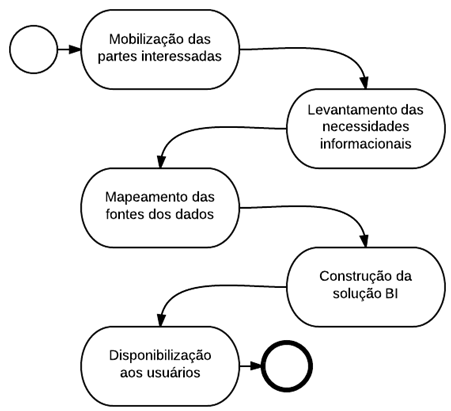
\includegraphics[width=0.6\textwidth]{./04-figuras/figura-04}
    \label{fig:ilustfig04}
\end{figure}
\vspace*{-0,9cm}
{\raggedright \fonte{Dispon\'{i}vel em: <https://canaltech.com.br>. Acesso em: 11 ago. 2020.}}\\

Essas cinco etapas constituem uma vis\~{a}o geral de todo o processo necess\'{a}rio para a completa implementa\c{c}\~{a}o e implanta\c{c}\~{a}o de uma solu\c{c}\~{a}o de BI. Todavia, a qualidade final do projeto de BI vai depender muito da aten\c{c}\~{a}o dada a cada uma dessas atividades, que descreveremos abaixo:

\begin{itemize}

    \item Mobiliza\c{c}\~{a}o das partes interessadas: para in\'{i}cio do projeto de BI, todos os \textit{stakeholders}\index{NewR}\footnote{Stakeholder: \'{e} um dos termos utilizados em diversas \'{a}reas como gest\~{a}o de projetos, comunica\c{c}\~{a}o social administra\c{c}\~{a}o e arquitetura de software referente \`{a}s partes interessadas que devem estar de acordo com as pr\'{a}ticas de governan\c{c}a corporativa executadas pela empresa.} devem ser mobilizados. Sem a participa\c{c}\~{a}o dos interessados, e principalmente do patroc\'{i}nio da alta gest\~{a}o, o BI provavelmente fracassar\'{a};
    
    \item Levantamento das necessidades informacionais: na atividade de levantamento das necessidades procuramos entender quais as informa\c{c}\~{o}es exigidas pelos gestores. Nessa etapa estamos procurando listar todas as solicita\c{c}\~{o}es sem nos preocupar, neste momento, com a exist\^{e}ncia "real" dos dados;
    
    \item Mapeamento das fontes dos dados: o mapeamento da origem dos dados \'{e} feito ap\'{o}s o levantamento das necessidades. Aqui \'{e} confrontando a viabilidade das solicita\c{c}\~{o}es efetuadas na etapa anterior. Caso afirmativo, s\~{a}o mapeadas as fontes dos dados para a posterior extra\c{c}\~{a}o na constru\c{c}\~{a}o do sistema de BI;
    
    \item Constru\c{c}\~{a}o da solu\c{c}\~{a}o BI: nessa etapa \'{e} iniciada a constru\c{c}\~{a}o propriamente dita da solu\c{c}\~{a}o. Se trata, sem dúvida alguma, da maior etapa do processo. Todas as atividades de extra\c{c}\~{a}o, qualidade dos dados, carga e teste das informa\c{c}\~{o}es s\~{a}o realizadas nesta etapa;
    
    \item Disponibiliza\c{c}\~{a}o aos usu\'{a}rios: depois de percorrido todas as etapas anteriores, chegamos, enfim \`{a} última etapa: disponibiliza\c{c}\~{a}o. Esta \'{e} uma etapa muito delicada, pois se trata do momento onde \'{e} entregue o produto de todo o esfor\c{c}o ao usu\'{a}rio final. Se a etapa de mobiliza\c{c}\~{a}o realizada no in\'{i}cio do processo tiver \^{e}xito, dificilmente teremos problemas na disponibiliza\c{c}\~{a}o. Nesta etapa, al\'{e}m de entregar a solu\c{c}\~{a}o, ser\'{a} feito toda a capacita\c{c}\~{a}o aos gestores e analistas que utilizar\~{a}o a ferramenta no dia a dia para a consulta de informa\c{c}\~{o}es de apoio \`{a}s decis\~{o}es.

\end{itemize}

Para construir um BI, primeiramente \'{e} feita a extra\c{c}\~{a}o e a an\'{a}lise dos dados da base ou das bases de dados, providos de uma gama de sistemas, os mesmos passam por um processo de transforma\c{c}\~{a}o (ETL).  

Faz-se uma limpeza deixando somente as informa\c{c}\~{o}es que ser\~{a}o úteis para a empresa. Ap\'{o}s esse processo de transforma\c{c}\~{a}o \'{e} criado os \textit{Data Marts}, ambos definidos na fase de implementa\c{c}\~{a}o, onde \'{e} feita a organiza\c{c}\~{a}o de todas as informa\c{c}\~{o}es. 

Analisando e correlacionando os dados onde posteriormente ser\~{a}o passados por outro processo de transforma\c{c}\~{a}o preparando-os para serem armazenados em um reposit\'{o}rio de dados denominado \textit{Data Warehouse}. 

Assim, quando os dados est\~{a}o no DW, todos organizados contendo somente as informa\c{c}\~{o}es relevante para o bom desenvolvimento da empresa \'{e} feita a explora\c{c}\~{a}o desses dados. 

Gerando informa\c{c}\~{o}es úteis para os usu\'{a}rios, sendo mostradas de diversas formas, atrav\'{e}s de gr\'{a}ficos, relat\'{o}rios entre outros, esse processo \'{e} feito utilizando as ferramentas OLAP, que nos oferece uma interface interativa com o usu\'{a}rio.

\section{As Principais fontes de dados}

As Fonte de dados \'{e} o local onde s\~{a}o armazenados os dados que ser\~{a}o coletados por programas de computador \textit{(softwares)} para ent\~{a}o serem transformados nas informa\c{c}\~{o}es que ir\~{a}o ajudar uma determinada \'{a}rea ou algumas \'{a}reas de neg\'{o}cio da sua empresa.

Alguns exemplos para que voc\^{e} entenda o que s\~{a}o fontes de dados:

\begin{itemize}

    \item Planilhas Eletrônicas (Excel);
    \item Banco de Dados;
    \item Arquivo CSV;
    \item Arquivo XML;
    \item Arquivos JSON;
    \item Documentos de texto (Bloco de Notas, Word, etc);
    \item Sistemas ERP;
    \item Sistemas CRM;
    \item Sociais, entre outras.
    
\end{itemize}

Conhecer e entender o que \'{e} uma fonte de dados \'{e} o ponto chave de todo o processo de implanta\c{c}\~{a}o de um BI, pois, deve-se ter certeza absoluta que os dados l\'{a} armazenados s\~{a}o \'{i}ntegros. N\~{a}o existe limite para fonte de dados, obviamente que quanto mais fontes (confi\'{a}veis) mais informa\c{c}\~{o}es e conhecimentos ser\~{a}o geradas, consequentemente mais detalhes do seu neg\'{o}cio voc\^{e} ter\'{a}. Nada adianta voc\^{e} ter 10 (dez) fontes de dados que n\~{a}o se pode confiar. 

\'{e} melhor voc\^{e} ter 2 (duas) fontes de dados com total certeza da integridade do que 10 (dez) em situa\c{c}\~{a}o duvidosa. As fontes de dados s\~{a}o a base do BI, pois s\~{a}o esses os dados que ser\~{a}o coletados e transformados em informa\c{c}\~{o}es que por sua vez ir\~{a}o gerar previs\~{o}es, an\'{a}lises, gr\'{a}ficos e relat\'{o}rios que ser\~{a}o a fonte de \textit{insights}\index{NewR}\footnote{\textit{Insight}: \'{e} o entendimento de uma causa e efeito espec\'{i}ficos dentro de um contexto espec\'{i}fico. O termo insight pode ter v\'{a}rios significados relacionados: um peda\c{c}o de informa\c{c}\~{a}o o ato ou resultado de entender a natureza interior das coisas ou de ver intuitivamente uma introspec\c{c}\~{a}o um peda\c{c}o de informa\c{c}\~{a}o; o ato ou resultado de entender a natureza interior das coisas ou de ver intuitivamente (chamado noesis em grego) uma introspec\c{c}\~{a}o; o poder da observa\c{c}\~{a}o e dedu\c{c}\~{a}o aguda , discernimento e percep\c{c}\~{a}o, chamado intelec\c{c}\~{a}o ou um entendimento de causa e efeito com base na identifica\c{c}\~{a}o de relacionamentos e comportamentos em um modelo, contexto ou cen\'{a}rio.} e a base para a tomada de decis\~{o}es de todos os colaboradores da organiza\c{c}\~{a}o.

\section{ETL (Extra\c{c}\~{a}o, Transforma\c{c}\~{a}o e Carga)}

Para \cite{dw-kimball-2013} o sistema de extra\c{c}\~{a}o, transforma\c{c}\~{a}o e carga (ETL) do ambiente DW/BI consiste em uma \'{a}rea de trabalho, estruturas de dados instanciadas e um conjunto de processos.

A extra\c{c}\~{a}o \'{e} a primeira etapa do processo de inser\c{c}\~{a}o de dados no ambiente de armaz\'{e}m de dados. Extrair significa ler e entender os dados de origem e copiar os dados necess\'{a}rios no sistema ETL para manipula\c{c}\~{a}o adicional. Neste ponto, os dados pertencem ao armaz\'{e}m de dados.

Depois que os dados s\~{a}o extra\'{i}dos para o sistema ETL, existem inúmeras transforma\c{c}\~{o}es em potencial, como limpeza dos dados (corre\c{c}\~{a}o de erros de ortografia, resolu\c{c}\~{a}o de conflitos de dom\'{i}nio, tratamento de elementos ausentes ou an\'{a}lise em formatos padr\~{a}o), combina\c{c}\~{a}o de dados de v\'{a}rias fontes e desduplicar dados. 

A etapa final do processo ETL \'{e} a estrutura\c{c}\~{a}o f\'{i}sica e o carregamento de dados nos modelos dimensionais alvo da \'{a}rea de apresenta\c{c}\~{a}o. Como a principal miss\~{a}o do sistema ETL \'{e} entregar as tabelas de dimens\~{o}es e fatos na etapa de entrega, esses subsistemas s\~{a}o cr\'{i}ticos.

Por outro lado, as tabelas de fatos s\~{a}o geralmente grandes e demoram para carregar, mas prepar\'{a}-las para a \'{a}rea de apresenta\c{c}\~{a}o \'{e} geralmente simples. 
Quando as tabelas de dimens\~{o}es e fatos em um modelo dimensional s\~{a}o atualizadas, indexadas, fornecidas com agregados apropriados e com garantia de qualidade adicional, a comunidade de neg\'{o}cios \'{e} notificada de que os novos dados foram publicados.

Ap\'{o}s validar os dados para conformidade com as regras de neg\'{o}cios definidas um-para-um e muitos-para-um, pode ser inútil dar o passo final da cria\c{c}\~{a}o de um banco de dados f\'{i}sico 3NF \textit{(Third Normal Form)}\index{NewR}\footnote{3NF (\textit{Third Normal Form} ou Terceira Forma Normal): \'{e} uma forma normal usada para normalizar um design de banco de dados para reduzir a duplica\c{c}\~{a}o de dados e garantir a integridade referencial, garantindo que: a entidade est\'{a} na segunda forma normal; Nenhum atributo n\~{a}o prim\'{a}rio (sem chave) depende transitivamente de qualquer chave, ou seja, nenhum atributo n\~{a}o prim\'{a}rio depende de outros atributos n\~{a}o primos. Todos os atributos n\~{a}o primos devem depender apenas das chaves candidatas.}, pouco antes de transformar os dados novamente em estruturas desnormalizadas para a \'{a}rea de apresenta\c{c}\~{a}o de BI.

Infelizmente, algumas iniciativas de DW/BI falharam miseravelmente, porque concentraram toda a sua energia e recursos na constru\c{c}\~{a}o de estruturas normalizadas, em vez de alocar tempo para o desenvolvimento de uma \'{a}rea de apresenta\c{c}\~{a}o dimensional que ofere\c{c}a suporte \`{a} melhor tomada de decis\~{o}es de neg\'{o}cios. 

Segundo \cite{dw-kimball-2013}, \'{e} aceit\'{a}vel criar um banco de dados normalizado para suportar os processos ETL; no entanto, esse n\~{a}o \'{e} o objetivo final. As estruturas normalizadas devem estar fora dos limites das consultas do usu\'{a}rio, pois elas derrotam os objetivos g\^{e}meos de compreensibilidade e desempenho. 

Em resumo a ETL \'{e} a respons\'{a}vel pela prepara\c{c}\~{a}o dos dados que far\~{a}o parte
do \textit{Data Warehouse} ou \textit{Data Mart}. Ela se d\'{a} basicamente em três passos: extra\c{c}\~{a}o, transforma\c{c}\~{a}o e carga de dados.

\begin{figure}[H]
	\vspace*{0,2cm}
    \centering
    \caption{ciclo de vida do ETL em todo seu processo.}
    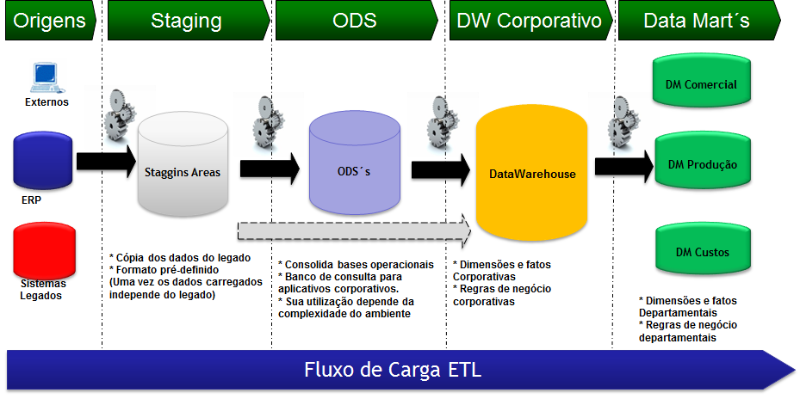
\includegraphics[width=0.6\textwidth]{./04-figuras/figura-05}
    \label{fig:ilustfig05}
\end{figure}
\vspace*{-0,9cm}
{\raggedright \fonte{Dispon\'{i}vel em: <https://https://www.igti.com.br>. Acesso em: 13 ago. 2020.}}\\

\section{\textit{Data Warehouse}}

O \textit{Data Warehouse} conforme \cite{si-inmon-1997} \'{e} o ponto central da arquitetura de processamento de informa\c{c}\~{o}es para sistemas de apoio \'{a} decis\~{a}o (SAD), visto que suportam o processamento informacional atrav\'{e}s de um alicerce s\'{o}lido de integra\c{c}\~{a}o de dados corporativos e hist\'{o}ricos para a realiza\c{c}\~{a}o de an\'{a}lises gerenciais.

De acordo com \cite{dw-kimball-2013}, um bom DW pode aliviar os sistemas de origem de grande parte da responsabilidade de representar o passado.

Segundo \cite{si-inmon-1997}, \textit{Data Warehouse} pode ser definido como uma cole\c{c}\~{a}o de dados orientados a assuntos, sendo eles integrados, n\~{a}o vol\'{a}teis e vari\'{a}veis em rela\c{c}\~{a}o ao tempo para apoio ao processo gerencial de tomada de decis\~{a}o.

Esta defini\c{c}\~{a}o acadêmica tr\'{a}s caracter\'{i}sticas importantes de um DW, que s\~{a}o melhor analisadas nas pr\'{o}ximas sess\~{o}es.

\subsection{Caracter\'{i}sticas}

Nas seguintes sess\~{o}es s\~{a}o apresentadas caracter\'{i}sticas de suma importância para um \textit{Data Warehouse}.

\subsubsection{Orienta\c{c}\~{a}o por assuntos}

A primeira caracter\'{i}stica not\'{a}vel do DW \'{e}a orientada por assunto, pois conforme Machado (2000), ela significa que o DW armazena as informa\c{c}\~{o}es agrupadas por assuntos de interesse da empresa que s\~{a}o de maior importância.

Tamb\'{e}m cabe salientar que segundo Machado (2000), os projetistas de DW devem ter seu foco na modelagem dos dados e no projeto de banco de dados. Sendo que em um DW somente importam os dados que sejam importantes para a tomada decis\~{a}o.

\subsubsection{Varia\c{c}\~{a}o tempos}

Conforme \cite{si-inmon-1997}, todos os dados no DW s\~{a}o precisos em algum instante no tempo. Esta caracter\'{i}stica b\'{a}sica dos dados do DW \'{e}muito diferente das encontradas em um ambiente operacional, pois nela quando se acessa uma unidade de dados, \'{e}esperado que esta reflita valores corretos no momento do acesso.

Em virtude de os dados no DW serem corretos como em algum momento no tempo, conforme \cite{si-inmon-1997} s\~{a}o ditos que estes variam com o tempo.

A varia\c{c}\~{a}o do tempo dos dados do DW segundo \cite{si-inmon-1997}) apresentam-se de diversas maneiras. Conforme \cite{bi-machado-2018}, a primeira e a mais simples \'{e}aquela que os dados representam informa\c{c}\~{o}es sobre espa\c{c}os de tempos de cinco a dez anos.

J\'{a} a segunda maneira s\~{a}o as estruturas b\'{a}sicas, onde cada estrutura cont\'{e}m um elemento tempo. E por fim a terceira maneira em que apresenta-se s\~{a}o os dados do DW, que uma vez armazenados corretamente, n\~{a}o podem ser atualizados \cite{si-inmon-1997}).

\subsubsection{N\~{a}o volatibilidadeos}

Conforme Inmon e Hackathorn (1997), outra caracter\'{i}stica definidora do DW trata-se do mesmo n\~{a}o ser vol\'{a}til. A manipula\c{c}\~{a}o b\'{a}sica dos dados em um DW \'{e}muito mais simples do que em ambientes operacionais, pois de acordo com Machado (2000) existem apenas dois tipos de opera\c{c}\~{o}es que podem ocorrer em um DW, a carga inicial do dados e o acesso em modo de leitura

\subsubsection{Integra\c{c}\~{a}oos}

Segundo Machado (2000), esta \'{e}uma das caracter\'{i}sticas de suma importância em um DW, pois todos os seus dados possuem um alto n\'{i}vel de integra\c{c}\~{a}o.
Conforme Inmon e Hackathorn (1997), os dados ao serem movidos de um ambiente operacional orientado a aplica\c{c}\~{o}es para o DW, s\~{a}o integrados antes de serem inclu\'{i}dos no DW. Estes mesmos autores afirmam tamb\'{e}m que os dados precisam ser armazenados no DW de uma forma única, mesmo quando as aplica\c{c}\~{o}es armazenam os dados de modo diferente.

\subsection{Granularidade de dados}

Conforme \cite{si-inmon-1997}, o aspecto mais importante do projeto de um \textit{Data Warehouse} faz referência a quest\~{a}o da granularidade, pois diz respeito ao n\'{i}vel de detalhe ou de resumo contido nas unidades de dados existentes no DW. Segundo Machado (2000), quanto mais detalhe, mais baixo o n\'{i}vel de granularidade, quanto menos detalhe, mais alto o n\'{i}vel de granularidade.

O motivo no qual torna a granularidade a principal quest\~{a}o do projeto, de acordo com \cite{si-inmon-1997} est\'{a} no fato de que ela afeta profundamente o volume de dados que encontra-se no DW e, ao mesmo tempo, afeta o tipo de consulta que pode ser atendida.

Segundo \cite{si-inmon-1997}, o n\'{i}vel de granularidade exerce um profundo efeito tanto sobre as perguntas que podem ser respondidas, bem como sobre os recursos necess\'{a}rios para responder a uma pergunta.

A escolha do n\'{i}vel ou n\'{i}veis de granularidade a serem utilizados em um projeto \'{e}indispens\'{a}vel para o sucesso. O m\'{e}todo mais indicado para definir os n\'{i}veis de granularidade conforme Machado (2000) est\'{a} na utiliza\c{c}\~{a}o do bom senso e da an\'{a}lise detalhada das necessidades de informa\c{c}\~{o}es levantadas para o projeto.
	
\subsection{Modelagem multidimensional}

Esta sess\~{a}o tem como objetivo apresentar conceitos e terminologias empregadas no processo de modelagem e na sequência deste trabalho. 

\subsubsection{Dimens\~{o}es}

Quando trata-se de dimens\~{a}o, est\'{a} se referindo aos elementos que participam de um fato, assunto de neg\'{o}cio. As dimens\~{o}es determinam o contexto de um assunto de neg\'{o}cios \cite{bi-machado-2018}.

As tabelas dimensionais conforme Kimball (1998), normalmente n\~{a}o possuem atributos num\'{e}ricos, uma vez que s\~{a}o somente textuais e classificat\'{o}rias dos elementos que participam de um fato.

Uma dimens\~{a}o de acordo com Machado (2000) pode conter membros e hierarquias. Os membros s\~{a}o uma classifica\c{c}\~{a}o de dados dentro de uma dimens\~{a}o. Estes membros de uma dimens\~{a}o podem ser arranjados em uma ou mais hierarquias, que por sua vez podem conter v\'{a}rios n\'{i}veis hier\'{a}rquicos.

\subsubsection{Fatos}

Segundo \cite{dw-kimball-2013}, a tabela de fatos em um modelo dimensional armazena as medidas de desempenho resultantes dos eventos do processo de neg\'{o}cios de uma organiza\c{c}\~{a}o.

O termo fato representa uma medida de neg\'{o}cios. Imagine estar no mercado observando os produtos sendo vendidos e anotando a quantidade de unidades e a quantidade de vendas em d\'{o}lar de cada produto em cada transa\c{c}\~{a}o de venda. 

Essas medidas s\~{a}o capturadas conforme os produtos s\~{a}o digitalizados no registro, conforme ilustrado na figura abaixo.

\begin{figure}[H]
	\vspace*{0,2cm}
    \centering
    \caption{Eventos de medi\c{c}\~{a}o de processo de neg\'{o}cios se traduzem em tabela de fato}
    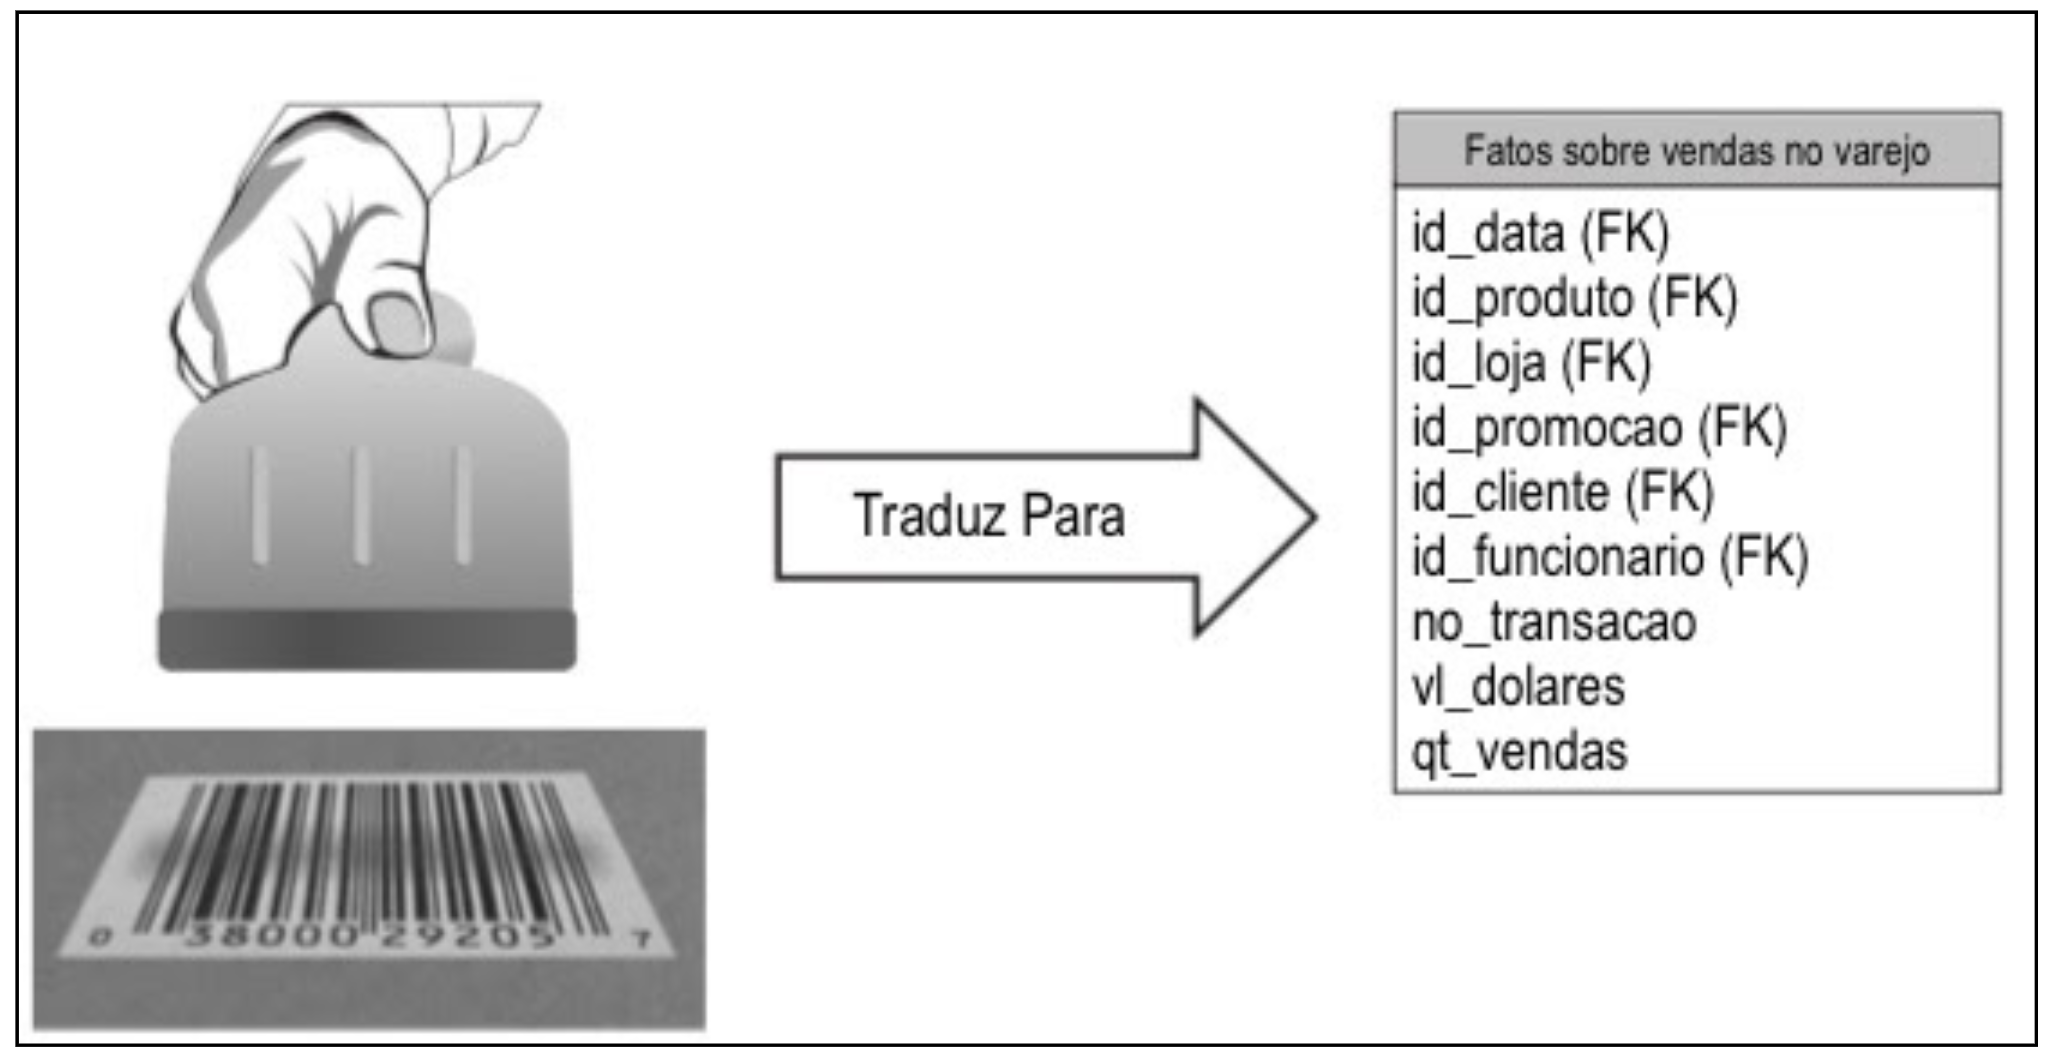
\includegraphics[width=0.6\textwidth]{./04-figuras/figura-06}
    \label{fig:ilustfig06}
\end{figure}
\vspace*{-0,9cm}
{\raggedright \fonte{adaptado de Kimball (2013)}}\\

\cite{bi-machado-2018}, conceitua que um fato trata-se de uma cole\c{c}\~{a}o de itens de dados, composta de dados de medidas e de contexto. Um fato consiste em um item de neg\'{o}cio, uma transa\c{c}\~{a}o de neg\'{o}cio ou um evento de neg\'{o}cio, nos quais se respondem as perguntas conforme figura 7. O mesmo \'{e}utilizado para verificar o processo de neg\'{o}cio de uma empresa.

De acordo com \cite{dw-kimball-1998}, tudo aquilo que reflete a evolu\c{c}\~{a}o dos neg\'{o}cios do dia-a-dia de uma institui\c{c}\~{a}o, \'{e}um fato.

\begin{figure}[H]
	\vspace*{0,2cm}
    \centering
    \caption{Fato}
    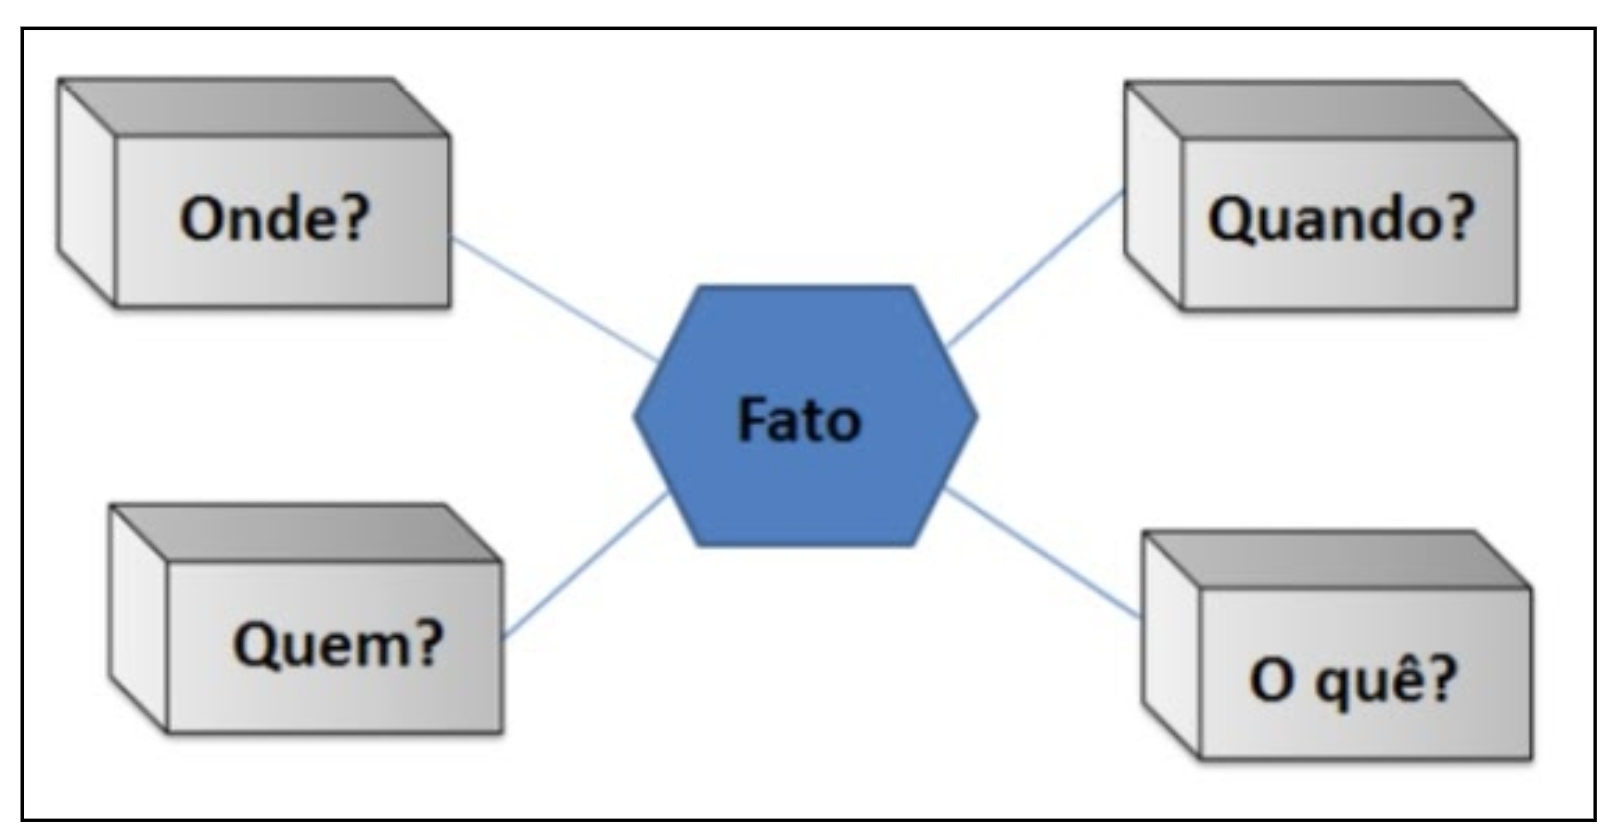
\includegraphics[width=0.6\textwidth]{./04-figuras/figura-07}
    \label{fig:ilustfig07}
\end{figure}
\vspace*{-0,9cm}
{\raggedright \fonte{adaptado de \cite{bi-machado-2018})}} \\

\subsubsection{Vari\'{a}veis}

As vari\'{a}veis ou medidas s\~{a}o os atributos num\'{e}ricos de um fato. Elas representam o desempenho de um indicador de neg\'{o}cios referente \`{a}s dimens\~{o}es que participam desse fato. Uma medida \'{e}estabelecida pela combina\c{c}\~{a}o das dimens\~{o}es que pertencem a um fato \cite{bi-machado-2018}.

\subsubsection{Opera\c{c}\~{o}es b\'{a}sicas}

Em um modelo de dados multidimensional se possu\'{i} opera\c{c}\~{o}es b\'{a}sicas de 
OLAP \textint{(On- Line Analytic Processing)}.

Conforme \cite{dw-kimball-1998}, OLAP \'{e}um termo inventado para descrever uma abordagem dimensional para o suporte \`{a} decis\~{a}o.

Estas opera\c{c}\~{o}es s\~{a}o usadas para analisar dados, sendo duas delas
:\textit{drill dow} e \textit{roll up}. Para poder-se utilizar estas opera\c{c}\~{o}es devesse fazer valer da granularidade (MACHADO, 2000).

Com a capacidade do \textit{drill down} se esta diminuindo o n\'{i}vel da granularidade, aumentando assim o n\'{i}vel de detalhes. De maneira oposta a isso, 
o \textit{roll up} aumenta o n\'{i}vel da granularidade, diminuindo desta maneira, o n\'{i}vel de detalhes das informa\c{c}\~{o}es.

\begin{figure}[H]
	\vspace*{0,2cm}
    \centering
    \caption{\textit{Drill Down} x  \textit{Roll Up}}
    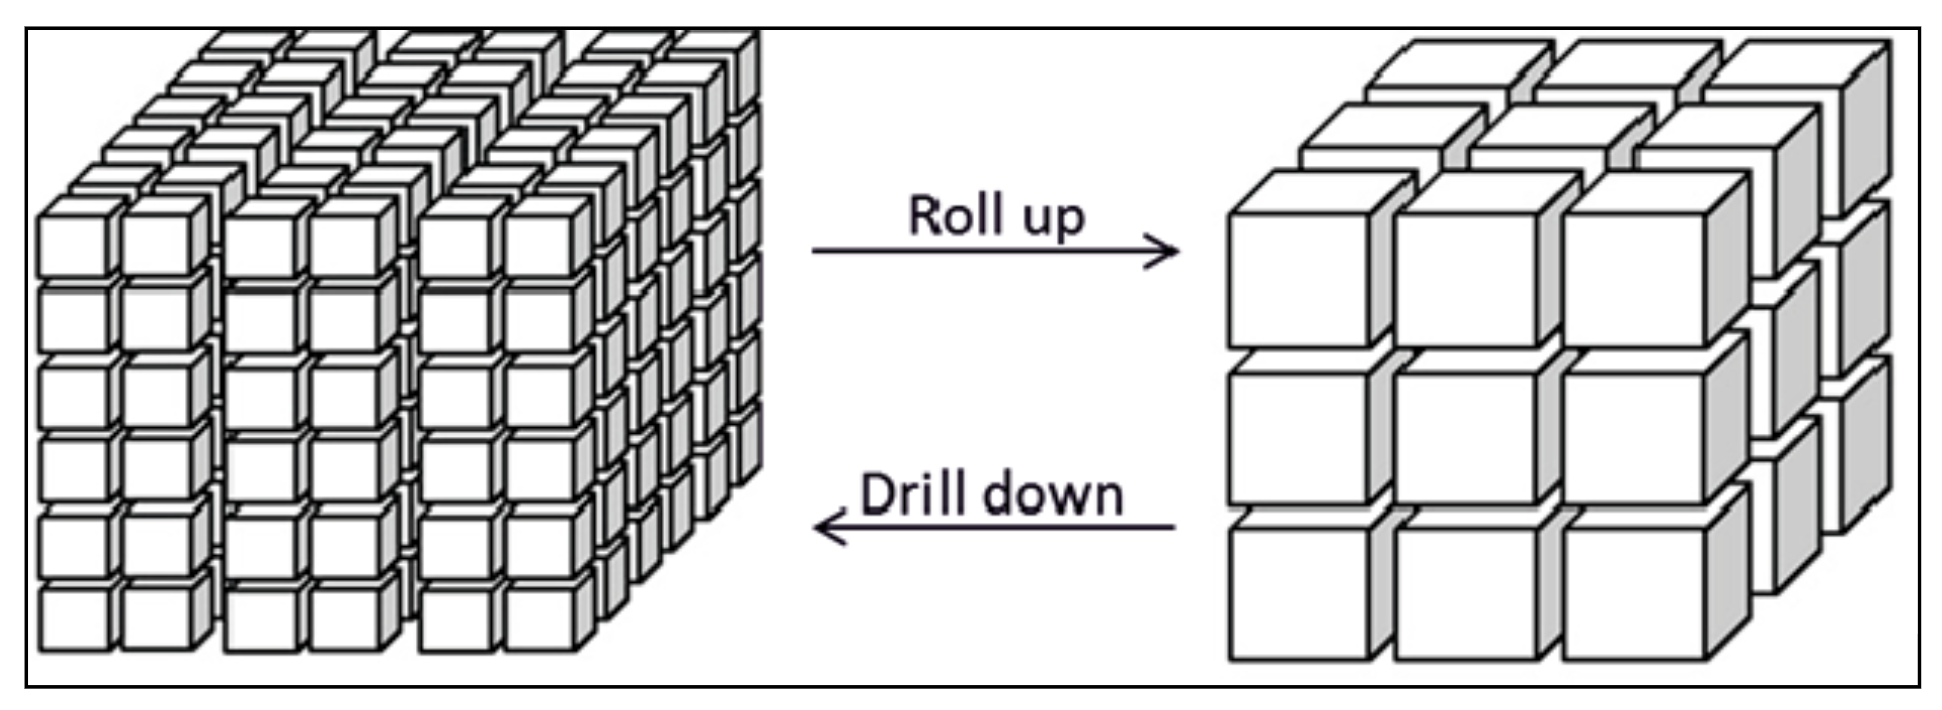
\includegraphics[width=0.6\textwidth]{./04-figuras/figura-08}
    \label{fig:ilustfig08}
\end{figure}
\vspace*{-0,9cm}
{\raggedright \fonte{Dispon\'{i}vel em: <https://(https://www.researchgate.net/figure/
Roll-up-and-Drill-down-operations-fig3-282320388>. Acesso em: 12 ago. 2020.}}\\

Portanto conforme \cite{bi-machado-2018}, estas opera\c{c}\~{o}es permitem movimentar nossa vis\~{a}o dos dados ao longo dos n\'{i}veis hier\'{a}rquicos de uma dimens\~{a}o.

\subsubsection{Modelo \textit{Star} (estrela)}

Em um modelo de dados multidimensional, a configura\c{c}\~{a}o que regula a organiza\c{c}\~{a}o dos fatos e das dimens\~{o}es para armazenamento corresponde geralmente, a um esquema em estrela \cite{bi-machado-2018}.

Este \'{e}composto por uma grande entidade central denominada tabela de fatos, e um conjunto de entidades menores denominadas tabelas de dimens\~{o}es, que por sua vez est\~{a}o organizadas ao redor da entidade central, formando assim uma estrela, conforme mostra a figura abaixo.

\begin{figure}[H]
	\vspace*{0,2cm}
    \centering
    \caption{Modelo Estrela}
    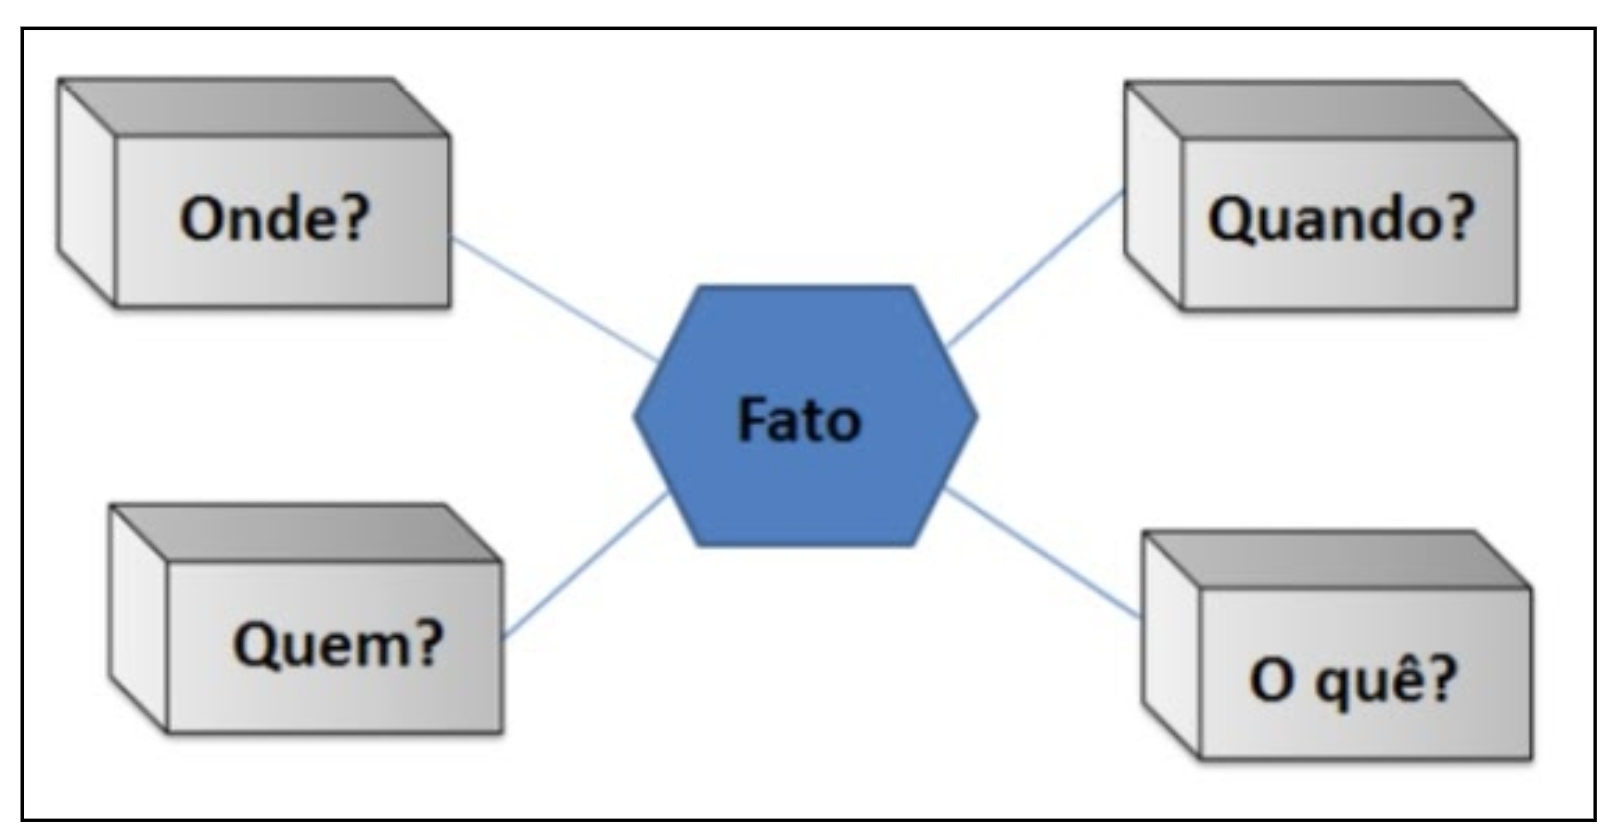
\includegraphics[width=0.6\textwidth]{./04-figuras/figura-09}
    \label{fig:ilustfig09}
\end{figure}
\vspace*{-0,9cm}
{\raggedright \fonte{adaptado de Machado (2000))}} \\

\subsubsection{Modelo \textit{Snowflake} (Floco de Neve)}

O modelo floco de neve da mesma forma que o modelo estrela possui uma entidade central denominada de fatos e um conjunto de entidades dimens\~{a}o ao seu redor formando uma estrela
.
No entanto o modelo floco de neve de acordo com \cite{bi-machado-2018}, \'{e}o resultado da decomposi\c{c}\~{a}o de uma ou mais dimens\~{o}es que possuem hierarquias entre seus membros. Conforme ilustrado na figura seguinte.
	
\begin{figure}[H]
	\vspace*{0,2cm}
    \centering
    \caption{Modelo Estrela}
    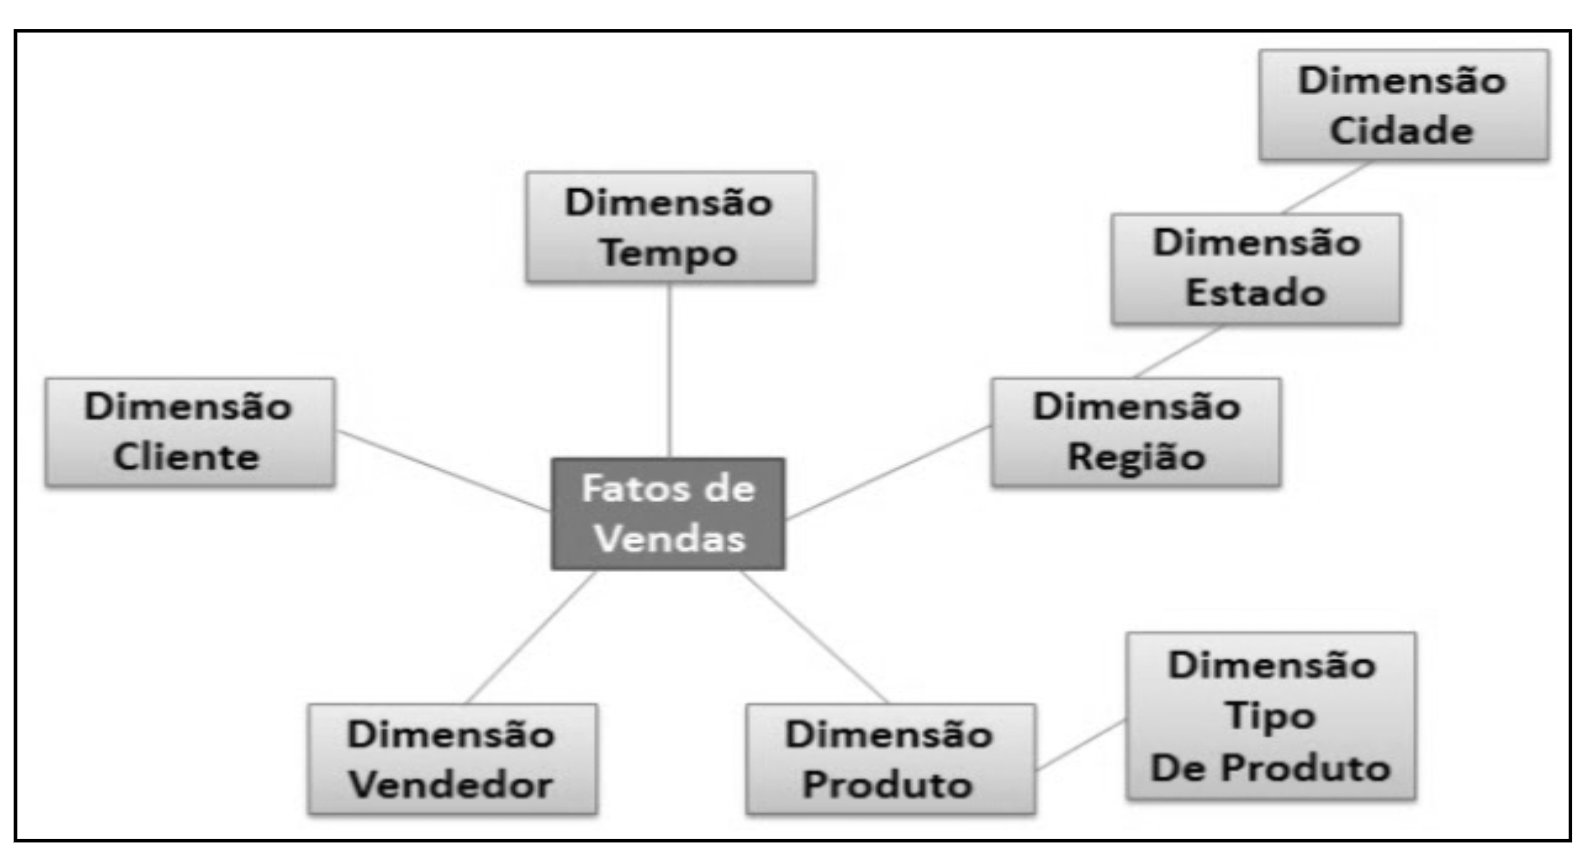
\includegraphics[width=0.6\textwidth]{./04-figuras/figura-10}
    \label{fig:ilustfig10}
\end{figure}
\vspace*{-0,9cm}
{\raggedright \fonte{adaptado de Machado (2000)}} \\

No entanto, conforme \cite{bi-machado-2018}, um DW n\~{a}o possui inclus\~{a}o de dados por meio de digita\c{c}\~{a}o, n\~{a}o necessitando assim garantir que os valores textuais sejam únicos, e nem t\~{a}o pouco se preocupar com a economia de espa\c{c}o, mas sim garantir o preceito de informa\c{c}\~{a}o r\'{a}pida.

O modelo floco de neve \'{e}esteticamente melhor para visualiza\c{c}\~{a}o de hierarquias, no entanto para se realizar consultas neste modelo s\~{a}o necess\'{a}rios mais joins, resultando assim em um gasto maior de tempo.
	
\section{\textit{Data Mart}}

Para \cite{si-inmon-1997}, um \textit{Data Mart} pode ser definido como um SGBD multidimensional que fornece uma estrutura bastante flex\'{i}vel de acesso a dados. Enquanto o DW extrai, transforma e limpa os dados dos sistemas transacionais, mantendo-os integrados em quantidades massivas e em seu n\'{i}vel mais baixo, o DM se serve destes dados, extraindo dados para um departamento ou uma \'{a}rea de neg\'{o}cio, oferecendo flexibilidade e controle ao usu\'{a}rio final, pois com o DM \'{e}poss\'{i}vel fatiar e agrupar dados de diversas maneiras.

Para \cite{bi-machado-2018} e \cite{dw-kimball-1998}, os dados do \textit{Data Mart} s\~{a}o direcionados a um departamento ou a uma \'{a}rea espec\'{i}fica do neg\'{o}cio e representam um subconjunto do DW corporativo.

O DM muitas vezes \'{e}visto como uma alternativa ao DW, pois custa menos e leva menos tempo para ser projetado e implementado. \'{e}criado para um grupo dirigido de usu\'{a}rios, normalmente um setor da empresa.

\section{KDD}

Extra\c{c}\~{a}o de conhecimento (tamb\'{e}m conhecido como processo KDD, do ingl\^{e}s 
\textit{(Knowledge Discovery in Databases)} \'{e} um processo de extra\c{c}\~{a}o de informa\c{c}\~{o}es de base de dados, que cria rela\c{c}\~{o}es de interesse que n\~{a}o s\~{a}o observadas pelo especialista no assunto, bem como auxilia a valida\c{c}\~{a}o de conhecimento extra\'{i}do.

Assim, segundo \cite{kdd-fayyad}, o KDD (\textit{Knowledge Discovery in Databases} ou Descoberta do conhecimento em Banco de Dados) \'{e} uma tentativa de solucionar o problema causado pela "era da informa\c{c}\~{a}o": sobre carga de dados.

Por\'{e}m, a difini\c{c}\~{a}o mais conhecida eo KDD, diz que ele \'{e}o processo, n\~{a}o trivial, de extra\c{c}\~{a}o de informa\c{c}\~{o}es impl\'{i}citas, previamente desconhecidas e potencialmente úteis, a partir dos dados armazenados em um banco de dados \cite{kdd-fayyad}.

O processo \'{e} n\~{a}o trivial , segundo \cite{kdd-fayyad}) j\'{a} que alguma t\'{e}cnica de busca ou infer\^{e}ncia \'{e} envolvida, ou seja, n\~{a}o \'{e} apenas um processo de computa\c{c}\~{a}o direta. 

Os padr\~{o}es descobertos devem ser v\'{a}lidos com algum grau de certeza, novos (para o sistema e de prefer\^{e}ncia tamb\'{e}m para o usu\'{a}rio), potencialmente úteis (trazer algum benef\'{i}cio) e compreens\'{i}veis (se n\~{a}o imediatamente ent\~{a}o depois da interpreta\c{c}\~{a}o).

O processo de busca de conhecimento cont\'{e}m uma s\'{e}rie de passos: sele\c{c}\~{a}o, pr\'{e}-processamento e limpeza, transforma\c{c}\~{a}o, minera\c{c}\~{a}o de dados (data mining) e interpreta\c{c}\~{a}o/avalia\c{c}\~{a}o. 

Simplificando, pode-se dizer que o processo de KDD compreende, na verdade, todo o ciclo que o dado percorre at\'{e} se transformar em informa\c{c}\~{a}o, conforme pode ser visto na figura abaixo.

\begin{figure}[H]
	\vspace*{0,2cm}
    \centering
    \caption{Ciclo dos dados em um KDD}
    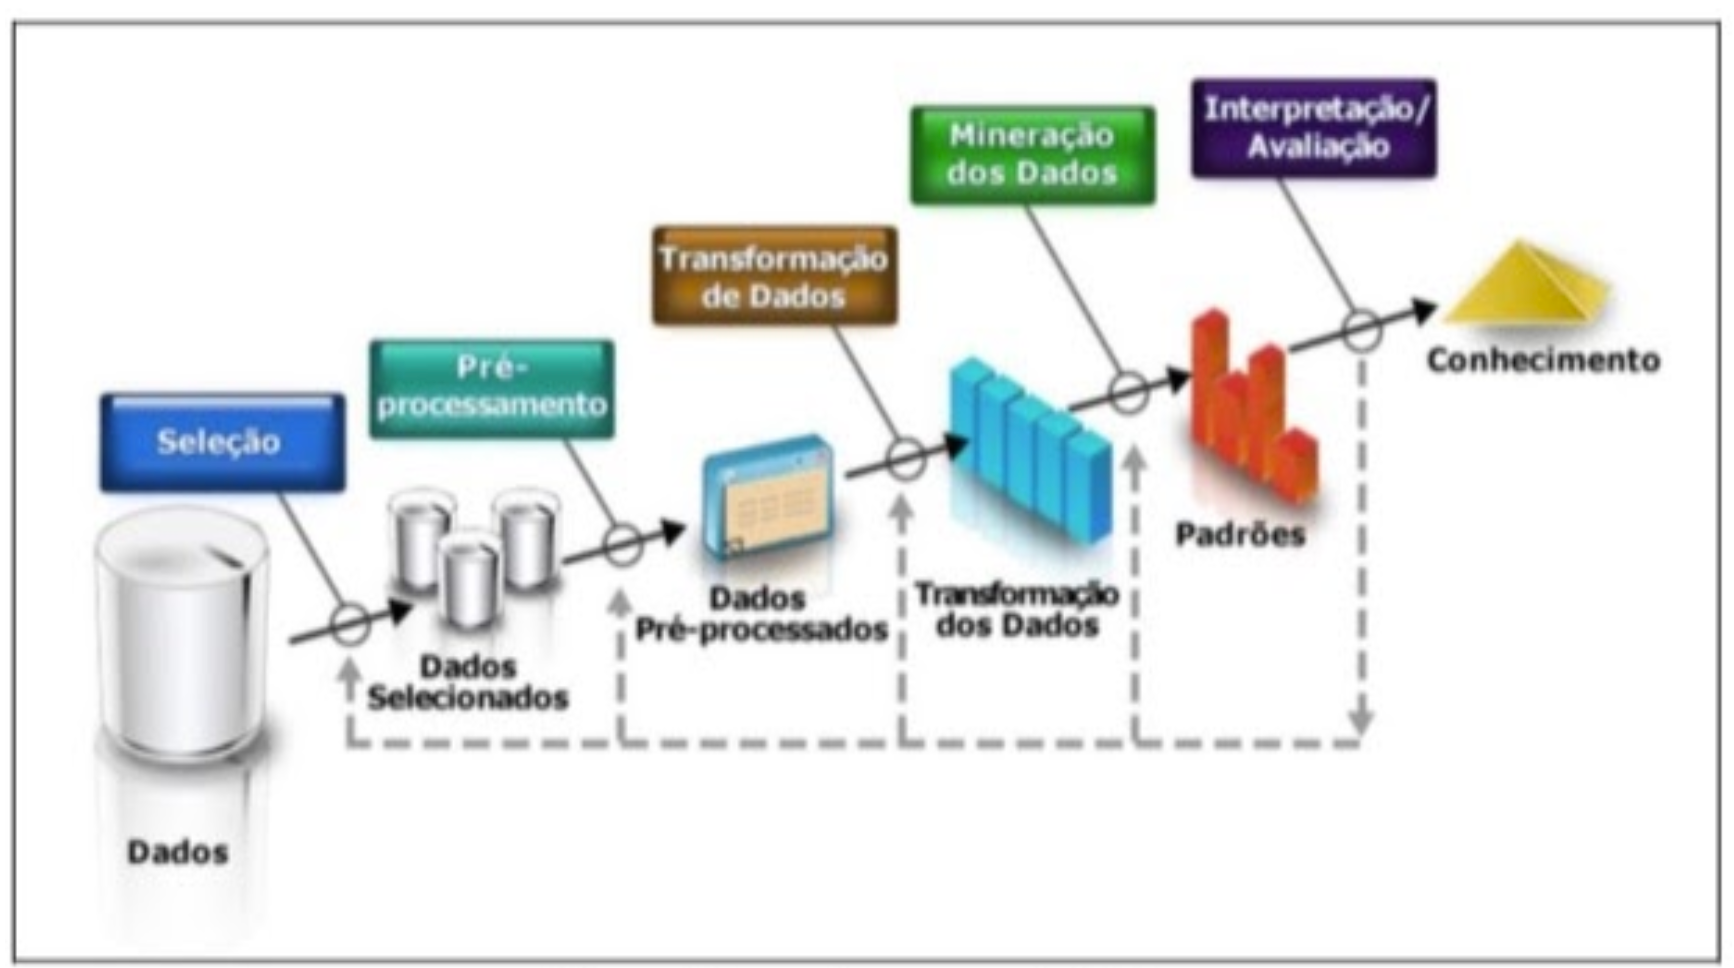
\includegraphics[width=0.6\textwidth]{./04-figuras/figura-11}
    \label{fig:ilustfig11}
\end{figure}
\vspace*{-0,9cm}
{\raggedright \fonte{adaptado de \cite{kdd-fayyad}}} \\

Suas caracter\'{i}sticas s\~{a}o:

\begin{itemize}

    \item N\~{a}o trivial j\'{a} que alguma t\'{e}cnica de busca ou infer\^{ê}ncia \'{e}envolvida (n\~{a}o \'{e}apenas um processo de computa\c{c}\~{a}o direta);
    
    \item Os padr\~{o}es descobertos devem ser v\'{a}lidos com algum grau de certeza, novos, trazer algum benef\'{i}cio e serem compreens\'{i}veis (se n\~{a}o imediatamente ent\~{a}o depois da interpreta\c{c}\~{a}o.

\end{itemize}

Em nosso trabalho n\~{a}o iremos objetivar o uso dessa tecnologia, pois, n\~{a}o \'{e} a nosso inten\c{c}\~{a}o, mas, foi preciso informar da sua exist\^{e}ncia nesse t\'{o}pico para que haja um aprofundamento te\'{o}rico de tudo que envolve o mundo do BI. 

O processo \'{e} iterativo e, embora apresente uma defini\c{c}\~{a}o semelhante tamb\'{e}m ao minera\c{c}\~{a}o de dados, deve ser composto de uma s\'{e}rie de etapas sequenciais, podendo haver retorno a etapas anteriores, isto \'{e}, as descobertas realizadas (ou a falta delas).

Eventualmente, este processo conduz a novas hip\'{o}teses e descobertas. Neste caso, o usu\'{a}rio pode decidir pela retomada dos processos de minera\c{c}\~{a}o, ou uma nova sele\c{c}\~{a}o de atributos, por exemplo, para validar as hip\'{o}teses que surgiram ao longo do processo.

O produto esperado da extra\c{c}\~{a}o de conhecimento \'{e} uma informa\c{c}\~{a}o relevante para ser utilizada pelos tomadores de decis\~{a}o. Alguns autores, por\'{e}m, defendem o ponto de vista de que o conhecimento descoberto n\~{a}o precisa necessariamente ser incorporado a um sistema de apoio \`{a} decis\~{a}o (SAD).

\section{OLAP (Processamento Anal\'{i}tico On-line)}

O OLAP \'{e}composto por inúmeras t\'{e}cnicas e ferramentas que possibilitam a explora\c{c}\~{a}o de dados armazenados em um data warehouse, utilizando t\'{e}cnicas que permitem a visualiza\c{c}\~{a}o de v\'{a}rios dados. 

Diariamente as organiza\c{c}\~{o}es acumulam grandes quantidades de dados e o OLAP as ajuda a fazer uma an\'{a}lise mais segura e confi\'{a}vel desse grande volume de dados transformando-os em informa\c{c}\~{o}es. (JACOBSON; MISNER, 2007).

O OLAP \'{e}composto por v\'{a}rios processos usados para criar, gerenciar e manipular os dados contido no banco de dados, o mesmo tem a fun\c{c}\~{a}o de agilizar a recupera\c{c}\~{a}o dos dados, podendo ainda executar e examinar uma grande quantidade de dados. 

Os gestores das empresas usam OLAP em qualquer setor da organiza\c{c}\~{a}o, pois lhes proporciona realizar an\'{a}lises comparativas para auxili\'{a}-los nas decis\~{o}es tomadas no dia-a-dia. (JACOBSON; MISNER, 2007).

Os sistemas OLAP s\~{a}o conhecidos por representar algumas caracter\'{i}sticas com:

\begin{itemize}
    
    \item Oferece aos usu\'{a}rios uma resposta \`{a}s suas consultas com mais rapidez. Apresenta relat\'{o}rios que antes eram dif\'{i}ceis de analisar devida sua complexidade de uma forma mais f\'{a}cil, simples de entender.
    
    \item O OLAP oferece ferramentas para que os usu\'{a}rios possam criar seus pr\'{o}prios relat\'{o}rios, com isso poder\'{a} analisar como anda o desenvolvimento das empresas de uma forma mais r\'{a}pida e flex\'{i}vel; \cite{bi-larson-2006};
    
    \item Oferece uma forma interativa com o usu\'{a}rio durante a disponibiliza\c{c}\~{a}o das informa\c{c}\~{o}es;
    
    \item Permite que haja uma repeti\c{c}\~{a}o de dados para melhorar as consultas;
    Permite que se fa\c{c}am c\'{a}lculos com uma complexidade alta e uma visualiza\c{c}\~{a}o desses c\'{a}lculos em diversas dimens\~{o}es; e;
    
    \item Permite que se fa\c{c}am ajustes para que as consultas se tornem mais segura, para que a partir desses resultados se possam concluir analises de tendências.

\end{itemize}

Uma organiza\c{c}\~{a}o, seja pública ou privada que usa OLAP ter\'{a} um desempenho melhor diante das concorrentes, pois com o uso dessa t\'{e}cnica pode trazer informa\c{c}\~{o}es com mais rapidez, da melhor forma para seu entendimento e tudo de uma forma bem interativa. 

Hoje no ambiente competitivo globalizado o que vale \'{e}ter informa\c{c}\~{a}o e estar sempre informado do que esta acontecendo no mundo, mas, principalmente, dentro de sua pr\'{o}pria empresa e essa t\'{e}cnica possibilita que todos os membros fiquem integrados do que acontece na organiza\c{c}\~{a}o de forma simples, r\'{a}pida e interativa. (JACOBSON; MISNER, 2007).

Segundo \cite{dw-kimball-2013} o mesmo, classifica os sistemas OLAP em ROLAP, MOLAP, HOLAP E DOLAP, essas ferramentas possibilitam diferentes formas de organizar os dados antes de apresent\'{a}-los ao usu\'{a}rio final.

A ROLAP \'{e}utilizada nas an\'{a}lises mais explorat\'{o}rias dos dados, sendo bastante utilizada pela \'{a}rea de marketing. 

Quanto \`{a} ferramenta MOLAP, permite an\'{a}lises mais simples e r\'{a}pidas, mas, tamb\'{e}m, apresenta limita\c{c}\~{a}o de tamanho, tendo estrutura similar ao de uma planilha, com linhas e colunas. \cite{olap-microsoft-2020}.

A HOLAP \'{e}o resultado da combina\c{c}\~{a}o entre as ferramentas MOLAP e ROLAP, extraindo o que h\'{a} de melhor das duas. \cite{olap-microsoft-2020}.

As ferramentas DOLAP \textit{(Desktop Online Analytical Processing)} disparam uma instru\c{c}\~{a}o
SQL \textit{(Structure Query Language)} de computador simples, configurado como cliente, com um servidor de dados que retorna um microcubo de informa\c{c}\~{o}es a serem analisadas no cliente, permitindo o processamento da m\'{a}quina cliente, sem problemas de tr\'{a}fego de rede e nem problemas de escalabilidade. 

Por\'{e}m existe uma desvantagem neste processo, o microcubo n\~{a}o deve ser muito grande para que n\~{a}o haja uma perda de largura de banda. (MICROSOFT CORPORATION, 2007)

\subsection{Tipos de opera\c{c}\~{a}o sobre OLAP}

Segundo \cite{olap-ballard-2006}, as principais opera\c{c}\~{o}es utilizadas nas ferramentas OLAP s\~{a}o : \textit{Drill Across, Drill Down, Drill Up, Drill Throught, Alertas, Ranking, Filtros, Sorts, Breaks, Slice and Dice e o pivot.}

\begin{itemize}

    \item \textit{Drill Across}: ocorre quando o usu\'{a}rio atravessa um n\'{i}vel intermedi\'{a}rio numa mesma dimens\~{a}o. Ex: Ele executa um Drill Across quando h\'{a} uma altera\c{c}\~{a}o de ano para mês diretamente;

    \item \textit{Drill Down}: ocorre quando o n\'{i}vel de detalhes da informa\c{c}\~{a}o sofre um aumento;
    
    \item \textit{Drill Up}: ocorre quando o usu\'{a}rio diminui o n\'{i}vel de detalhes da informa\c{c}\~{a}o, \'{e}o contrario do Drill Down;
    
    \item \textit{Drill Throught}: ocorre quando o usu\'{a}rio muda a informa\c{c}\~{a}o de dimens\~{a}o. Ex: Est\'{a}s na dimens\~{a}o tempo e no pr\'{o}ximo passo est\'{a}s analisando a informa\c{c}\~{a}o por regi\~{a}o (outra dimens\~{a}o);
    
    \item Alertas: servem para informar sobre as situa\c{c}\~{o}es importantes e mostrar os valores mediante as condi\c{c}\~{o}es;
    
    \item \textit{Ranking}: possibilita juntar todos os resultados por ordem decrescente ou crescente, baseando-se em objetos num\'{e}ricos conhecidos como as Measures;
    Filtros: d\~{a}o as permiss\~{o}es para os usu\'{a}rios aperfei\c{c}oarem, as pesquisas (Query) solicitadas por mais de uma vez, como se fossem filtros de informa\c{c}\~{o}es;
    
    \item \textit{Sorts}: serve para ordenar as informa\c{c}\~{o}es de forma crescente ou decrescente, de acordo com a escolha do usu\'{a}rio;
    
    \item \textit{Breaks}: serve para agrupar as informa\c{c}\~{o}es em blocos. Ex: O usu\'{a}rio que ver as informa\c{c}\~{o}es por cidades, ent\~{a}o ele executou um break. Ap\'{o}s esta a\c{c}\~{a}o ter sido executada, as informa\c{c}\~{o}es estar\~{a}o agrupadas por cidades;
    
    \item \textit{Slice and Dice}: como o OLAP gera ou recupera um micro-cubo, o Slice and Dice têm a responsabilidade de fazer altera\c{c}\~{a}o na posi\c{c}\~{a}o de uma informa\c{c}\~{a}o, alterar linhas e colunas para facilitar a compreens\~{a}o dos usu\'{a}rios e girar o cubo sempre que tiver necessidade, esse recurso faz parte das principais caracter\'{i}sticas da ferramenta;
    
    \item \textit{Pivot}: Permite a troca de linhas por colunas em uma tabela ou modifica\c{c}\~{a}o da posi\c{c}\~{a}o das dimens\~{o}es em um gr\'{a}fico. Ou seja, \'{e} o ângulo pelo qual os dados s\~{a}o visualizados.
    
\end{itemize}

Conforme \cite{dw-kimball-2013}, o OLAP \'{e}uma tecnologia de banco de dados que foi otimizada para consulta e relat\'{o}rio, em vez de processamento de transa\c{c}\~{o}es. Os dados de origem do OLAP s\~{a}o bancos de dado OLTP\textit{(Online Transactional Processing)} que s\~{a}o comumente armazenados em um \textit{Data Warehouse}.

Os dados OLAP s\~{a}o originados a partir desses dados hist\'{o}ricos, e integrados em estruturas que permitem an\'{a}lise sofisticada, sendo organizados hierarquicamente e armazenados em cubos em vez de tabelas. Esta tecnologia \'{e}organiza de forma f\'{a}cil as estruturas multidimensionais para agilizar o acesso aos dados a serem analisados. 

Logo, s\~{a}o a base dos relat\'{o}rios de tabelas ou gr\'{a}ficos dinâmicos, e a exibi\c{c}\~{a}o de resumos de alto n\'{i}vel, bem como a exibi\c{c}\~{a}o de resultados detalhistas.

\subsection{Os componentes do OLAP}

Os tipos de dados que constituem os bancos de dados OLAP s\~{a}o as medidas e as dimens\~{o}es, sendo as medidas, os dados num\'{e}ricos, ou seja, as quantidades e m\'{e}dias que você usa para tomar decis\~{o}es comerciais, e as dimens\~{o}es s\~{a}o as categorias que você usa para organizar essas medidas.

Os bancos de dados OLAP auxiliam na organiza\c{c}\~{a}o dos dados por muitos n\'{i}veis de detalhe, utilizando algumas categorias que ser\~{a}o descritas a seguir: (MICROSOFT CORPORATION, 2007).

\begin{itemize}

    \item Cubo: s\~{a}o formas de dados que ajudam na realiza\c{c}\~{a}o de an\'{a}lises, sem eles n\~{a}o seria poss\'{i}vel realizar an\'{a}lises de dados em diversas dimens\~{o}es. Eles possibilitam combinar o tempo, a geografia e os produtos com números de vendas de forma r\'{a}pida, eficiente e resumida, mais detalhes sobre cubo no t\'{o}pico 2.9;
    
    \item Medida: s\~{a}o todos os valores num\'{e}ricos encontrados na regi\~{a}o central de um cubo, como por exemplo, as vendas, os lucros, as receitas e os custos, todos processados, agregados e analisados;
    
    \item Membro: \'{e} caracterizado por objetos que podem desempenhar um ou mais impacto de dados em uma hierarquia;
    Membro calculado: o valor de um membro \'{e}calculado enquanto esta ocorrendo uma execu\c{c}\~{a}o por meio de uma express\~{a}o. O valor de um membro calculado pode ser originado do valor de outro membro;
    
    \item Dimens\~{a}o: \'{e} composta por uma ou mais hierarquias organizadas de n\'{i}veis em um cubo de uma forma que o usu\'{a}rio possa entender e assim us\'{a}-las para fazer an\'{a}lise de dados;
    
    \item Hierarquia: \'{e}uma forma de ordena\c{c}\~{a}o em diferentes n\'{i}veis organizando os membros de uma dimens\~{a}o de forma que cada membro tenha um possa ter um membro pai e zero ou at\'{e}mais membros filho. De acordo com a hierarquia o membro filho \'{e}inferior ao membro atual, j\'{a} o pai est\'{a} em um n\'{i}vel superior relacionado diretamente ao membro atual. O valor pai \'{e}no gera consolidado aos valores de todos os seus filhos;
    
    \item N\'{i}vel: em um processo hier\'{a}rquico, os dados podem ser ordenados em n\'{i}veis de detalhe inferiores e superiores, como por exemplo, Ano, Semestre, Trimestre, Mês e Dia em uma hierarquia Tempo.

\end{itemize}

\subsection{As Aplica\c{c}\~{o}es do OLAP}

O OLAP \'{e}caracterizado por ser diversificado, podendo ser aplicado em diversos setores de uma organiza\c{c}\~{a}o como no setor de: (MICROSOFT CORPORATION, 2007)

\begin{itemize}

    \item Nas finan\c{c}as: nesse setor com o uso de OLAP poder\'{a} ser realizada uma analise de balan\c{c}o geral da empresa, fazer um or\c{c}amento, fluxo de caixa da empresa, contas \`{a} receber;
    \item Nas vendas: pode ser feita uma an\'{a}lise das vendas escolhendo a regi\~{a}o, os produtos que mais foram vendidos nesta regi\~{a}o, o vendedor respons\'{a}vel pelas vendas, entre outros dados;
    \item No \textit{Marketing}: o OLAP possibilita que fa\c{c}a uma an\'{a}lise de mercados, lucratividade de produto, e fazer uma an\'{a}lise de pre\c{c}o ou volume;
    \item Nos Recursos Humanos: com os sistemas OLAP poder\'{a} ser feito uma an\'{a}lise de benef\'{i}cios, fazer proje\c{c}\~{a}o de sal\'{a}rios e analise de números de funcion\'{a}rios da empresa ou do setor; e;
    \item Na Manufatura: atrav\'{e}s dessa ferramenta OLAP pode-se gerenciar o estoque da empresa, os fornecedores, fazer planejamento de que produtos est\~{a}o em demanda, analisar os custos dos materiais para fabrica\c{c}\~{a}o dos produtos.

\end{itemize}

\subsection{As Ferramentas OLAP}

Os gestores das organiza\c{c}\~{o}es tem a necessidade de uma ferramenta que os auxiliem na explora\c{c}\~{a}o dos dados que forne\c{c}a informa\c{c}\~{o}es confi\'{a}veis, que de acordo com a an\'{a}lise das mesmas possam os auxiliar na tomada de decis\~{a}o. Para isso existem algumas ferramentas que poder\~{a}o ajuda-los nesse processo de explora\c{c}\~{a}o e analise dos dados como o \textit{Mondrian} ou textit{Schema Workbench} , que ser\'{a} tema de um t\'{o}pico especifico, e que faz parte do Pentaho.

\section{Cubo}

Segundo Carlo Vercellis (VERCELLIS, 2009), o projeto de DW e data mart s\~{a}o baseados em um paradigma multidimensional para a representa\c{c}\~{a}o de dados que fornece grandes vantagens no momento da consulta de dados, ele pode garantir tempo de resposta r\'{a}pida, mesmo em complexas consultas, enquanto no lado l\'{o}gico, as dimens\~{o}es naturalmente correspondem a crit\'{e}rios normais e facilmente entend\'{i}veis a usu\'{a}rios para realizarem suas an\'{a}lises.

A representa\c{c}\~{a}o multidimensional \'{e}baseada em um esquema em estrela que cont\'{e}m os dois tipos de tabelas de dados, as dimens\~{o}es e Fatos.
Com isso pode-se dizer que um cubo, \'{e}a estrutura multidimensional de dados que expressa a forma na qual os tipos de informa\c{c}\~{o}es se relacionam entre si. \'{e}formado pela tabela Fato e pelas tabelas de dimens\~{a}o que a circundam e representam poss\'{i}veis formas de visualizar e consultar os dados (VERCELLIS, 2009).

Pode-se citar um exemplo de um cubo atrav\'{e}s de um conjunto de lojas, considerando o faturamento de um produto em um mês do ano, em uma loja. Na existência de um cubo tridimensional, uma dimens\~{a}o representa os produtos, a outra o per\'{i}odo e outra as lojas. A figura 12,  representa o exemplo.

% figuras
\begin{figure}[H]
	\vspace*{0,2cm}
    \centering
    \caption{Cubo}
    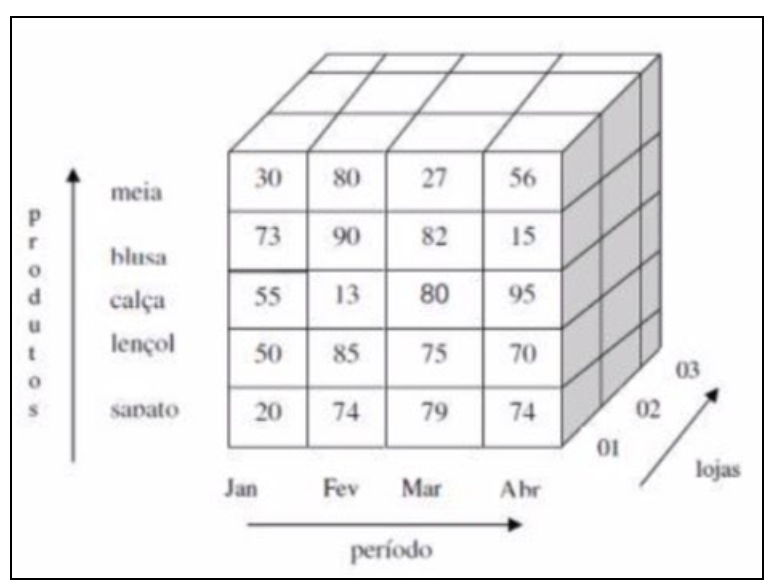
\includegraphics[width=0.6\textwidth]{./04-figuras/figura-12}
    \label{fig:ilustfig12}
\end{figure}
\vspace*{-0,9cm}
{\raggedright \fonte{VERCELLIS (2009)}} \\

\section{\textit{Data mining} (minera\c{c}\~{a}o de dados)}

Alguns profissionais da \'{a}rea de an\'{a}lise de informa\c{c}\~{a}o enfrentam problemas no processo de transformar dados que as empresas acumulam em suas transa\c{c}c\~(oo)es di\'{a}rias em informa\c{c}\~{o}es que ser\~{a}ao de grande utilidade para o desempenho dos neg\'{o}ocios. 

Assim, Segundo CORTES, o \textit{Data Mining} \'{e}um processo feito sobre enormes reposit\'{o}rios de dados como o \textit{data warehouse} buscando identificar padr\~{o}es e alguma rela\c{c}\~{a}o de consumo que n\~{a}o s\~{a}o conhecidos pela empresa e que podem ser usados na tomada de decis\~{a}o. (C\^{O}RTES, 2008).

Usando o \textit{Data Mining} esse problema ser\'{a} resolvido, pois ele \'{e}um processo pelo qual se descobri informa\c{c}\~{o}es importantes para a empresa, como os padr\~{o}es, as associa\c{c}\~{o}es entre as informa\c{c}\~{o}es da base de dados, mudan\c{c}as, anomalias e as estruturas, em grandes quantidades de dados que s\~{a}o armazenados em base de dados ou outros reposit\'{o}rios de dados. (C\^{O}RTES, 2008)
